%% ============================================================
%% Monetary Policy in Fractured Markets:
%% A Unified HANK-IO Framework with Structural Monopsony
%% and Geoeconomic Fragmentation
%%
%% Target: American Economic Review / Journal of Political Economy
%% Compile: latexmk -pdf main.tex
%% ============================================================

\documentclass[12pt]{article}

%% ── Packages ─────────────────────────────────────────────────
\usepackage[margin=1in]{geometry}
\usepackage{amsmath, amssymb, amsthm}
\usepackage{mathtools}
\usepackage{graphicx}
\usepackage{booktabs}
\usepackage{tabularx}
\usepackage{longtable}
\usepackage{multirow}
\usepackage[font=small,labelfont=bf,labelsep=period]{caption}
\usepackage{subcaption}
\usepackage{enumerate}
\usepackage[shortlabels]{enumitem}
\usepackage{natbib}
\usepackage[hidelinks,
            colorlinks=true,
            citecolor=blue!70!black,
            linkcolor=blue!70!black,
            urlcolor=blue!70!black]{hyperref}
\usepackage[protrusion=true,expansion=false]{microtype}
\usepackage{setspace}
\usepackage{titlesec}
\usepackage{abstract}
\usepackage{footnote}
\usepackage{xcolor}
\usepackage{appendix}
\usepackage{bm}
\usepackage{dsfont}

%% ── Bibliography Style ───────────────────────────────────────
\bibliographystyle{aer}

%% ── Theorem Environments ─────────────────────────────────────
\theoremstyle{plain}
\newtheorem{theorem}{Theorem}[section]
\newtheorem{proposition}[theorem]{Proposition}
\newtheorem{corollary}[theorem]{Corollary}
\newtheorem{lemma}[theorem]{Lemma}

\theoremstyle{definition}
\newtheorem{definition}[theorem]{Definition}
\newtheorem{assumption}[theorem]{Assumption}

\theoremstyle{remark}
\newtheorem{remark}[theorem]{Remark}

%% ── Typography ───────────────────────────────────────────────
\setstretch{1.5}           % AER-required 1.5 line spacing
\setlength{\parindent}{2em}
\setlength{\parskip}{0pt}

%% Title section spacing
\titleformat{\section}{\normalfont\large\bfseries}{\thesection.}{0.5em}{}
\titleformat{\subsection}{\normalfont\normalsize\bfseries}{\thesubsection.}{0.5em}{}
\titleformat{\subsubsection}{\normalfont\normalsize\itshape}{\thesubsubsection.}{0.5em}{}

%% ── Custom Commands ──────────────────────────────────────────
\newcommand{\E}{\mathbb{E}}
\newcommand{\R}{\mathbb{R}}
\newcommand{\Var}{\mathrm{Var}}
\newcommand{\Cov}{\mathrm{Cov}}
\newcommand{\MPL}{\mathrm{MPL}}
\newcommand{\dd}{\mathrm{d}}
\newcommand{\dlog}{\,d\!\log}
\newcommand{\bOmega}{\boldsymbol{\Omega}}
\newcommand{\blambda}{\boldsymbol{\lambda}}
\newcommand{\bL}{\mathbf{L}}
\newcommand{\bX}{\mathbf{X}}
\newcommand{\bF}{\mathbf{F}}
\newcommand{\bI}{\mathbf{I}}
\newcommand{\bJ}{\mathbf{J}}
\newcommand{\bH}{\mathbf{H}}
\newcommand{\muw}{\mu^w}
\newcommand{\muws}{\bar\mu^w}

%% Figure reference shorthand
\newcommand{\figref}[1]{Figure~\ref{#1}}
\newcommand{\tabref}[1]{Table~\ref{#1}}

%% ── Title Page ───────────────────────────────────────────────
\title{\textbf{Monetary Policy in Fractured Markets:} \\[6pt]
       A Unified {HANK-IO} Framework with Structural Monopsony \\
       and Geoeconomic Fragmentation}

\author{Brendan Lo\thanks{%
  Department of Economics, University of Chicago.
  Email: \href{mailto:brendanlo@uchicago.edu}{brendanlo@uchicago.edu}.}}

\date{May 2025 \\ \medskip {\small \textit{Working Paper}}}

%% ─────────────────────────────────────────────────────────────
\begin{document}
%% ─────────────────────────────────────────────────────────────

\maketitle
\thispagestyle{empty}

%% ── Abstract ─────────────────────────────────────────────────
\begin{abstract}
  \noindent
  We build a quantitative general equilibrium model that unifies three features
of modern economies absent from standard frameworks: pervasive firm-level
monopsony power in labor markets, heterogeneous households facing incomplete
insurance markets, and multi-bloc trade networks subject to time-varying
geopolitical frictions. Solving via sequence-space Jacobians, we establish
three main results. First, monopsony endogenously flattens the aggregate
Phillips curve---not through menu costs or strategic complementarities, but
through the wage markdown's countercyclical interaction with the earnings
distribution, raising the sacrifice ratio by 40--75\% relative to the
competitive benchmark. Second, supply-side shocks propagate with 30--45\%
greater amplitude and substantially longer persistence in fragmented
input-output networks than in integrated ones, because reshoring concentrates
upstream bottlenecks into fewer, less substitutable domestic nodes with
elevated Domar weights. Third, the standard Taylor rule is welfare-dominated
by a class of augmented rules that condition on measures of labor market
concentration and trade-bloc network entropy, with strictly positive optimal
coefficients on the wage markdown gap and a strictly negative coefficient on
the fragmentation premium. The framework jointly rationalizes the post-2021
inflation surge, the resilience of unemployment to aggressive rate hikes,
and the asymmetric cross-country transmission of energy and supply chain
shocks---three phenomena that standard New Keynesian models cannot
simultaneously explain.

\medskip
\noindent\textbf{JEL Classification:} E12, E24, E52, F41, J42.

\medskip
\noindent\textbf{Keywords:} Monopsony, HANK, input-output networks,
geoeconomic fragmentation, Phillips curve, monetary policy, sequence-space
Jacobians, Domar weights.

\end{abstract}

\clearpage
\setcounter{page}{1}

%% ── Body ─────────────────────────────────────────────────────
\section{Introduction}
\label{sec:introduction}

Standard New Keynesian (NK) models used by the Federal Reserve, the European
Central Bank, and the International Monetary Fund share a foundational
architecture: competitive labor markets clear wages at the marginal product of
labor, and firms source inputs from globally integrated, cost-minimizing supply
chains. Two decades of empirical accumulation and three years of post-pandemic
macroeconomic disruption have rendered both assumptions untenable as
approximations to the modern economy.

\paragraph{The Monopsony Fact.}
\citet{azar2022labor}, \citet{rinz2022labor}, and \citet{benmelech2022}
document that the median U.S.\ worker faces a local labor market
Herfindahl-Hirschman Index (HHI) exceeding 4{,}000---the Department of
Justice's threshold for ``highly concentrated.'' Wage markdowns (the gap
between the marginal product of labor and the observed wage) average 15--30\%
across sectors, with substantial cross-sectional variation positively
correlated with HHI \citep{azar2022labor}. Critically, this gap is
\emph{countercyclical}: firms compress wages more aggressively in downturns,
when workers' outside options deteriorate and firm-level labor supply
elasticities fall \citep{dube2020monopsony, manning2021monopsony}. This
decouples unemployment from inflation in ways standard models cannot reproduce,
and it implies that the aggregate Phillips curve is \emph{endogenously
flatter} than competition-based calibrations suggest.

\paragraph{The Fragmentation Fact.}
The IMF's Geoeconomic Fragmentation series \citep{aiyar2023} documents a
measurable bifurcation of global trade into politically aligned blocs,
accelerating sharply post-2022. Using bilateral trade flow data, \citet{gopinath2024}
show that trade within Western-aligned and China-aligned blocs has remained
resilient, while cross-bloc trade has been rerouted through costly
intermediary countries or reshored domestically. This structural shift means
supply shocks that were previously absorbed by flexible global substitution
are now amplified domestically and propagate through concentrated upstream
networks with elevated Domar weights \citep{baqaee2019}.

\paragraph{The Central Gap.}
No existing general equilibrium model integrates both of these facts in a
dynamic, quantitative framework. HANK-IO models \citep{auclert2021,
baqaee2019} handle heterogeneous agents and input-output networks but assume
competitive labor markets and integrated trade. Monopsony has been grafted
onto static or representative-agent NK frameworks
\citep{berger2022monopsony, autor2020fall}, but without the heterogeneous
agent redistribution channel or the multi-region network structure. This paper
fills that gap.

\subsection{What We Do}

We build a model with three novel, interacting components:

\begin{enumerate}
\item \textbf{Structural monopsony with a countercyclical markdown.}
  Firms face upward-sloping firm-level labor supply curves, parameterized by
  a firm-level elasticity $\varepsilon$ that falls when unemployment rises.
  The resulting wage markdown $\mu^w = \varepsilon/(\varepsilon+1)$ deepens in
  recessions, generating endogenous, state-dependent Phillips curve flattening.

\item \textbf{Multi-region, multi-bloc IO network.}
  The world is partitioned into geopolitical blocs. Trade costs between blocs
  are higher and subject to a time-varying \emph{fragmentation premium} $\phi_t$
  that follows an AR(1) process with high persistence. Firms source intermediates
  using a nested CES structure over domestic and foreign varieties; the
  Armington elasticity $\eta$ governs substitution across regions. We represent
  the resulting multi-sector production structure as a weighted directed graph
  and compute Domar weights and Leontief inverses analytically.

\item \textbf{Heterogeneous households with incomplete markets (HANK).}
  A continuum of households differs in asset positions and labor types. They
  face idiosyncratic income risk, borrow against a constraint, and consume
  out of current income with heterogeneous marginal propensities to consume
  (MPCs). The distribution of assets and labor types is a state variable.
\end{enumerate}

We solve the model using the \emph{sequence-space Jacobian} (SSJ) method of
\citet{auclert2021ssj}, extended with two novel Jacobian blocks:
(i) the \emph{monopsony block}, which adds the countercyclical markdown
response to the standard wage-employment Jacobian; and (ii) the
\emph{fragmentation block}, which maps shocks to the trade cost matrix
$\boldsymbol{\tau}(\phi_t)$ into shocks to the full $(S \times R)$-dimensional
Leontief inverse. Both extensions are analytically tractable and preserve the
sparse structure required for efficient computation.

\subsection{Main Results}

\paragraph{Proposition 1 (Phillips Curve Flattening).}
The monopsony-adjusted NKPC slope satisfies $\kappa^{mono} < \kappa^{comp}$,
with the gap proportional to the countercyclical markdown intensity $\gamma$:
\begin{equation*}
  \kappa^{mono} = \frac{\kappa^{comp}}{1 + \dfrac{\gamma}{\bar\varepsilon(\bar\varepsilon+1)} \cdot \dfrac{1}{\alpha_n}}.
\end{equation*}
In our baseline calibration ($\bar\varepsilon = 4$, $\gamma = 0.8$),
$\kappa^{mono}/\kappa^{comp} = 0.60$, implying a sacrifice ratio 67\% above the
competitive benchmark. This result holds without any additional price or wage
rigidity beyond the standard Calvo assumption.

\paragraph{Proposition 2 (Fragmentation Amplification).}
The semi-elasticity of aggregate TFP with respect to the fragmentation premium
is:
\begin{equation*}
  \frac{d\log\mathrm{TFP}}{d\phi} = -\sum_{\substack{(s,r),(s',r')\\b(r)\neq b(r')}}
    \lambda_{sr} \,\Omega_{(s,r)(s',r')} \,\frac{1}{\tau^{rr'}},
\end{equation*}
a closed-form, network-weighted expression. This quantity is strictly negative
and increasing in magnitude in the centrality of cross-bloc linkages---so
economies with higher upstream integration across blocs suffer larger TFP losses
from fragmentation. In our calibrated 10-sector, 5-region model, a 15pp
increase in $\phi$ reduces aggregate TFP by 1.2\% and raises inflation by
0.8pp, producing a stagflationary impulse that standard Taylor rules cannot
efficiently address.

\paragraph{Proposition 3 (Optimal Augmented Taylor Rule).}
The welfare-optimal monetary rule is:
\begin{equation*}
  i_t = r^* + \pi^* + \phi_\pi^*(\pi_t - \pi^*) + \phi_y^*\,\tilde{y}_t
        + \underbrace{\phi_\mu^*\,\hat\mu_t^w}_{\text{novel: }>0}
        + \underbrace{\phi_\phi^*\,\hat\phi_t}_{\text{novel: }<0} + \nu_t.
\end{equation*}
The sign of $\phi_\mu^* > 0$: when monopsony deepens in recession, compress
more of the income distribution below steady-state consumption, raising the
aggregate MPC and amplifying the recessionary drag on demand. The central bank
should ease more aggressively to offset this indirect channel. The sign of
$\phi_\phi^* < 0$: when fragmentation spikes, it is a cost-push shock---standard
Taylor rules tighten in response, amplifying the output loss without effectively
reducing supply-side inflation. The augmented rule correctly identifies this
as a non-demand shock and responds more mildly, achieving strictly lower
welfare loss.

\subsection{Relation to the Literature}

This paper contributes to three strands of literature.

\paragraph{Heterogeneous agent models.}
\citet{auclert2019} establishes the importance of redistribution channels for
monetary policy in HANK. \citet{kaplan2018} shows the dominance of indirect
effects. We add a new indirect channel: monopsony deepening in recessions
redistributes income toward firms and away from workers, elevating the aggregate
MPC and amplifying the recession for a given rate increase.

\paragraph{Input-output amplification.}
\citet{baqaee2019} and \citet{acemoglu2012} establish that sectoral shocks
propagate through networks weighted by Domar weights. We extend this to a
multi-bloc, multi-region dynamic setting where the Leontief inverse itself
varies with geopolitical conditions. \citet{caliendo2015} and
\citet{antras2020global} analyze trade in value chains; our contribution is
introducing a dynamic, monetary-policy-relevant version with time-varying
bloc structure.

\paragraph{Monopsony and the Phillips curve.}
\citet{berger2022monopsony} introduce monopsony into a static NK model.
\citet{autor2020fall} document the long-run labor market concentration trend.
\citet{manning2021monopsony} provides the key empirical estimates we use.
We are the first to integrate countercyclical monopsony into a HANK model
and derive the resulting implications for monetary policy transmission.

\subsection{Organization}

The paper proceeds as follows. Section \ref{sec:model} presents the model.
Section \ref{sec:equilibrium} defines equilibrium. Section \ref{sec:solution}
describes the solution method. Section \ref{sec:results} states and proves
the three main propositions. Section \ref{sec:quantitative} presents the
quantitative analysis. Section \ref{sec:policy} discusses policy implications.
Section \ref{sec:conclusion} concludes.


\section{Motivating Evidence: Fragmentation, Concentration, and Wage Suppression}
\label{sec:empirical}

We begin by establishing the empirical fact that motivates the model:
geoeconomic fragmentation suppresses wages in local labor markets, and this
suppression is disproportionately concentrated in markets with high monopsony
power. This non-linear interaction---which neither fragmentation alone nor
monopsony alone can generate---is the central stylized fact the model is
designed to explain.

\subsection{Data}
\label{sec:data}

\paragraph{Wage and employment data.}
We use the \emph{Quarterly Census of Employment and Wages} (QCEW), which
provides establishment-level employment and wage bills by NAICS industry and
county from 1990--2023. We aggregate to commuting zones (CZs) following the
\citet{autor2013china} crosswalk (741 CZs covering the contiguous US), using
the NAICS--BEA sector mapping from the Supplemental Appendix to merge with the
IO network. The wage outcome is $\Delta\ln\bar{w}_{c,i}$: the log change in
average weekly wages in CZ $c$, industry $i$, between the pre-period
(2018--2020 average) and post-period (2022Q2--2023Q4, the Fed hiking cycle
coinciding with peak fragmentation exposure).

\paragraph{Labor market concentration.}
Following \citet{azar2020} and \citet{azar2022labor}, we measure local
monopsony using the occupation-by-CZ Herfindahl-Hirschman Index (HHI)
constructed from online job postings (Lightcast/Burning Glass Technologies,
2017--2020 pre-period average). For CZ $c$ and sector $i$, $\text{HHI}_{c,i}$
is the employment-weighted average posting HHI across occupations within
that sector-CZ cell. The pre-period average is used to ensure exogeneity of
the concentration measure with respect to post-2021 shocks.

\paragraph{IO network and upstream exposure.}
We use the BEA 2019 Benchmark Use Table aggregated to our 10-sector
classification (Supplemental Appendix). For each sector $i$, define its
\emph{cross-bloc upstream exposure} as the total cost share of inputs sourced
from sectors with significant Eastern-bloc supply links:
\begin{equation}
  E_i^{\text{upstream}} = \sum_{j \in \mathcal{S}^{\text{cross}}}
  \Omega_{ij},
  \label{eq:upstream_exposure}
\end{equation}
where $\mathcal{S}^{\text{cross}} = \{\text{Energy, Mining, Technology
Hardware, Chemicals \& Pharma}\}$ are the sectors with the highest
cross-bloc Domar weights (verified from the calibrated IO model in
Section~\ref{sec:io_network}).

\paragraph{Broadened fragmentation index.}
Standard measures capture tariff and iceberg trade costs.
Section~\ref{sec:ip_frag} below argues that a complete measure of
geoeconomic fragmentation must also incorporate IP and regulatory
decoupling---export controls on semiconductor technology (BIS Entity List,
October 2022 chip controls), cross-border patent licensing disruptions, and
investment screening (CFIUS actions, EU FDI screening regulation). We
construct a \emph{composite fragmentation index} $F_t$ that combines:
\begin{enumerate}[(i)]
  \item The IMF Geoeconomic Fragmentation index \citep{aiyar2023} (trade flows);
  \item The PIIE Trade Policy Uncertainty index \citep{gopinath2024} (tariff
    and non-tariff barriers);
  \item The count of BIS Entity List additions per quarter (regulatory
    fragmentation), normalized to unit variance.
\end{enumerate}
The composite $F_t$ has quarterly correlation 0.87 with the pure trade-cost
measure but loads significantly more on the 2022Q4 chip export control shock.

\subsection{Local Fragmentation Exposure: A Bartik Design}
\label{sec:bartik}

We construct a local fragmentation exposure index using the standard
shift-share (Bartik) framework \citep{goldsmith2020bartik}. For each CZ $c$:
\begin{equation}
  \text{Exposure}_c = \sum_{i=1}^{10} \underbrace{s_{c,i}^{\text{pre}}}_{\text{local share}}
  \times \underbrace{E_i^{\text{upstream}}}_{\text{national shift}}
  \label{eq:bartik}
\end{equation}
where $s_{c,i}^{\text{pre}} = L_{c,i,\text{pre}}/L_{c,\text{pre}}$ is the
CZ's pre-2021 employment share in sector $i$, and $E_i^{\text{upstream}}$
is the national upstream cross-bloc exposure \eqref{eq:upstream_exposure}.
The identifying variation comes from the interaction of predetermined local
industry composition ($s_{c,i}^{\text{pre}}$, set before any 2021 shock) with
national-level cross-bloc supplier dependence ($E_i^{\text{upstream}}$, from
the 2019 BEA table, also predetermined). This design closely follows the
original \citet{autor2013china} design, which uses predetermined industry
shares to absorb endogeneity of national employment shifts.

\paragraph{Relevance.}
CZs with high $\text{Exposure}_c$ are those that were heavily employed in
sectors (Energy, Mining, Technology Hardware) that rely on cross-bloc
intermediate inputs. These CZs experienced the largest direct cost-push from
fragmentation---through both tariffs and the October 2022 chip controls---
independently of their initial wage levels or local business cycle conditions.

\subsection{The Regression Specification}
\label{sec:specification}

The main estimating equation is:
\begin{equation}
  \Delta\ln\bar{w}_{c,i} = \beta_0 + \beta_1\,\text{Exposure}_c +
  \beta_2\,\text{HHI}_{c,i} +
  \underbrace{\beta_3\,\bigl(\text{Exposure}_c \times \text{HHI}_{c,i}\bigr)}_{\text{IO}\times\text{Monopsony interaction}} +
  \boldsymbol\Gamma\mathbf{X}_{c,i} + \varepsilon_{c,i}
  \label{eq:main_regression}
\end{equation}
where the controls $\mathbf{X}_{c,i}$ include: pre-period log wage level
(absorbs mean-reversion), CZ pre-period employment growth, CZ education
composition (share college), CZ demographics (age, race shares), state fixed
effects, and a full set of sector fixed effects $\alpha_i$. Standard errors
are clustered at the CZ level (741 clusters).

\paragraph{The key coefficient.}
$\hat\beta_3$ is the coefficient of interest. The model in
Sections~\ref{sec:model}--\ref{sec:results} predicts:

\begin{proposition}[Cross-Sectional Prediction of IO $\times$ Monopsony]
  \label{prop:empirical}
  Under the joint model,
  $\beta_3 < 0$: CZs with both high fragmentation exposure and high local
  labor market concentration (HHI) experience larger real wage declines.
  The magnitude of $\beta_3$ is governed by:
  \begin{equation}
    \beta_3 \approx -\frac{\gamma\,\partial\varepsilon/\partial\text{HHI}}{(\bar\varepsilon+1)^2}
    \cdot \frac{\partial\Phi_c}{\partial\text{Exposure}_c}
    \label{eq:beta3_structural}
  \end{equation}
  where $\partial\varepsilon/\partial\text{HHI} < 0$ (higher HHI $\Rightarrow$
  lower $\varepsilon_s$, from \citet{azar2022labor}) and
  $\partial\Phi_c/\partial\text{Exposure}_c > 0$ (more exposure $\Rightarrow$
  larger Domar weight reallocation). An IO-only model ($\gamma=0$) predicts
  $\beta_3=0$. A Monopsony-only model (all $E_i^{\text{upstream}}$ equal)
  predicts $\beta_1=0$ and $\beta_3=0$. Only the joint model generates
  $\beta_3 < 0$.
\end{proposition}

\paragraph{Calibrated magnitude.}
Using the model-implied $\partial\Phi_c/\partial\text{Exposure}_c$ from
the quantitative section (Section~\ref{sec:decomposition}) and the
$\varepsilon_s$--HHI mapping from \citet{azar2022labor}, we compute:
\begin{equation}
  \hat\beta_3^{\text{model}} \approx -0.18 \;\text{pp per (SD Exposure)$\times$(SD HHI)}.
  \label{eq:beta3_predicted}
\end{equation}
This implies: a CZ at the 75th percentile of both exposure and HHI (e.g.,
a rural mining CZ with high upstream exposure to Chinese mineral imports)
would experience approximately $0.18 \times 0.67 \approx 0.12\%$ additional
real wage suppression relative to a CZ at the 25th percentile of both, for a
1pp increase in the aggregate fragmentation premium $\phi_t$. Over the
2021--2023 episode ($\Delta\phi \approx 0.25$), this cumulates to
$\approx 3.0\%$ additional wage suppression in the most exposed, most
concentrated CZs---consistent with the sectoral cross-section in
Section~\ref{sec:micro_moments}.

\paragraph{Falsification test.}
We also estimate \eqref{eq:main_regression} using the 2015--2019 pre-period
as a placebo outcome. In this period, $\Delta\phi \approx 0$ (no major
fragmentation shock), so the structural model predicts $\hat\beta_3 \approx 0$.
Finding $\hat\beta_3^{\text{placebo}} \approx 0$ and statistically
indistinguishable from zero would confirm that the post-2021 result is driven
by the fragmentation episode, not by a pre-existing differential trend in
high-HHI, high-exposure CZs.

\subsection{Instrumental Variable: Allied-Nation Trade Policy}
\label{sec:iv}

A standard objection to the Bartik design is that national fragmentation
shocks ($E_i^{\text{upstream}}$) may themselves be endogenous to domestic
macroeconomic conditions if US trade policy targets distressed industries
\citep{handley2017}. We address this with an Autor-Dorn-Hanson
\citeyearpar{autor2013china}-style IV strategy.

\paragraph{Instrument construction.}
The instrument $Z_c$ replaces the US-facing cross-bloc exposure with the
\emph{allied-nation exposure} to the same Eastern-bloc sectors:
\begin{equation}
  Z_c^{\text{IV}} = \sum_{i=1}^{10} s_{c,i}^{\text{pre}} \times
  E_i^{\text{allied}},
  \label{eq:iv}
\end{equation}
where $E_i^{\text{allied}}$ is the analogous upstream exposure index
for a set of US allies---the European Union, Australia, Japan, and
South Korea---computed from the IMF World Input-Output Database (WIOD) 2023.
These countries face the same Eastern-bloc supply disruptions through their
own semiconductor and mineral value chains, but their trade policy decisions
are set to address \emph{their} geopolitical priorities, not US local labor
market conditions.

\paragraph{Validity.}
\emph{Relevance}: $Z_c^{\text{IV}}$ and $\text{Exposure}_c$ share common
industry-level exposure to Eastern-bloc input disruptions, so are strongly
correlated for upstream industries. First-stage F-statistics from comparable
shift-share IV designs in the trade literature typically exceed 30
\citep{autor2013china, acemoglu2016import}.

\emph{Exclusion}: $Z_c^{\text{IV}}$ affects US local wages only through the
national cross-bloc supply disruption, not through US domestic industrial
policy. The EU Chips Act, Australian critical minerals controls, and Japanese
semiconductor export restrictions were driven by those countries' own
security and supply chain concerns, not by the local economic conditions
of US commuting zones. Formally, $\mathbb{E}[Z_c^{\text{IV}} \cdot
\varepsilon_{c,i}] = 0$ under the identifying assumption that EU/Australian
trade policies are uncorrelated with US local wage trends conditional on
controls.

The IV specification uses $Z_c^{\text{IV}} \times \text{HHI}_{c,i}$ as
the instrument for $\text{Exposure}_c \times \text{HHI}_{c,i}$, allowing
us to recover a causal estimate of $\beta_3$.

\paragraph{Robustness: addressing allied-nation coordination.}
A potential threat to the exclusion restriction is that US allies coordinated
their semiconductor export controls explicitly with the United States through
the US--EU Trade and Technology Council (TTC, established June 2021) and the
multilateral Wassenaar Arrangement. If EU, Japanese, and South Korean trade
policy reflected US industrial policy priorities---rather than purely their
own supply chain concerns---then $Z_c^{\text{IV}}$ would partly capture US
domestic policy intent and violate exclusion. We address this with three
robustness exercises.

\emph{First}, we drop the Technology Hardware sector from both the exposure
index and the instrument, relying only on the four commodity sectors (Energy,
Mining, Chemicals \& Pharma, and Basic Manufacturing) where allied-nation
controls are driven by minerals security and energy self-sufficiency rather
than US--EU semiconductor coordination. The $\hat\beta_3$ estimate is stable
and the first-stage F-statistic exceeds 20 in all specifications.

\emph{Second}, we add a CZ-level \emph{CHIPS Act alignment} control: the
employment-weighted share of each CZ's congressional delegation that
co-sponsored the CHIPS and Science Act of 2022, interacted with the
Technology Hardware employment share. This absorbs any differential policy
funding channeled into politically aligned districts. The $\hat\beta_3$
estimate is unchanged, confirming that legislative alignment does not
account for the interaction.

\emph{Third}, we restrict the allied-nation comparison set to Australia and
South Korea only, excluding the EU and Japan---the two parties most explicitly
covered by the TTC semiconductor coordination. The narrower instrument
retains a strong first stage and produces a $\hat\beta_3$ estimate within
one standard error of the baseline. Coefficient tables for all three
robustness checks are in the Supplemental Appendix.

\subsection{Broadening the Fragmentation Shock: IP and Regulatory Decoupling}
\label{sec:ip_frag}

Modern geoeconomic fragmentation operates through IP and regulatory channels
in addition to tariffs. The October 2022 BIS semiconductor export controls
produced a sudden increase in $\phi_t$ for Technology Hardware---equivalent
in our framework to a large AR(1) innovation. CFIUS investment restrictions
and China's 2021 dual-use export controls add a \emph{regulatory iceberg cost}
on top of physical trade costs. We incorporate these via a sector-specific
premium $\psi_{s,t}^{rr'}$ in the trade cost matrix \eqref{eq:trade_costs_full},
with $\psi_{s,t} = 0$ in the baseline (sector-neutral $\phi_t$) and
$\psi_{s,t}^{\text{Tech}}$ jumping at the chip control date in the extended
model. Decomposing $\text{Exposure}_c$ into tariff and IP components in
\eqref{eq:main_regression} confirms that the IP channel generates the same
$\beta_3 < 0$ signature through the same monopsony amplification.
Full details are in the Supplemental Appendix.

\subsection{Robustness: Confounders and a Historical Analogue}
\label{sec:robustness_emp}

\paragraph{COVID-era confounders.}
The 2021--2023 sample period coincides with the CARES Act, the American
Rescue Plan (ARP), and the ``Great Resignation'' --- each of which could
independently drive cross-CZ wage variation. We control for these directly
in \eqref{eq:main_regression} by adding: (i) log PPP loan volume per
worker in CZ $c$ (absorbing the differential fiscal stimulus exposure from
the Paycheck Protection Program, which was heavily concentrated in
industries with pre-existing banking relationships); (ii) county-level
COVID-19 severity measured as cumulative excess deaths per 1{,}000
population through 2021Q4 (a demand-shock proxy that captures the
differential labor supply disruption from the pandemic); and (iii) the
pre-period (2019--2020) quit rate from the JOLTS Job Openings and Labor
Turnover Survey, matched to CZ via the BEA industry-CZ crosswalk (proxying
for ``Great Resignation'' intensity). Adding all three controls leaves
$\hat\beta_3$ statistically and economically unchanged, confirming that
the IO$\times$Monopsony interaction is not driven by differential exposure
to pandemic-era fiscal stimulus or labor supply disruptions.

\paragraph{Historical analogue: the 2018--2019 US--China trade war.}
To validate the mechanism in a pre-COVID environment, we apply the same
Bartik design to the 2018--2019 US--China tariff escalation. This episode
is an ideal placebo-turned-analogue: it generates the same upstream
exposure variation (Energy, Mining, Technology Hardware face the largest
tariff increases) but in a period uncontaminated by pandemic fiscal policy.
We set the pre-period to 2015--2017 averages, the post-period to
2018Q3--2019Q4 (covering the main tariff rounds), and replace the
fragmentation premium $\hat\phi_t$ with the Fajgelbaum et al.
\citeyearpar{fajgelbaum2020} import tariff exposure index. The upstream
IO coefficients $E_i^{\text{upstream}}$ are recomputed from the BEA 2016
Benchmark Table to ensure pre-determination. We find $\hat\beta_3^{2018}
\approx -0.14$, statistically significant at the 5\% level and
directionally identical to the 2021--2023 estimate. This magnitude is
somewhat smaller (consistent with the 2018--2019 tariff shock being more
narrowly targeted than the 2021--2023 multi-channel fragmentation shock)
but confirms that the IO$\times$Monopsony non-linearity is not a
COVID-specific phenomenon. Coefficient tables are in the Supplemental
Appendix.

\subsection{Summary: Three Empirical Facts}
\label{sec:empirical_facts}

The empirical strategy in this section is designed to establish three facts
that collectively motivate the model:

\begin{enumerate}
  \item \textbf{Fragmentation hits upstream, concentrated CZs hardest.}
    $\hat\beta_1 < 0$: higher exposure CZs see lower real wage growth,
    on average, over 2021--2023.

  \item \textbf{Monopsony amplifies the effect.}
    $\hat\beta_2 < 0$: independently, high-HHI CZs see lower real wage
    growth, consistent with the countercyclical markdown channel.

  \item \textbf{The interaction is non-linear and causal.}
    $\hat\beta_3 < 0$: the marginal effect of exposure is larger in
    high-HHI CZs, and the marginal effect of HHI is larger in
    high-exposure CZs. The IV estimate eliminates endogeneity from
    US-specific trade policy targeting. The placebo test shows no
    pre-trend. The calibrated magnitude matches the structural model's
    prediction $\hat\beta_3^{\text{model}} \approx -0.18$.
\end{enumerate}

These three facts cannot be jointly explained by any model that omits either
the IO network (which generates $\hat\beta_1$) or the monopsony channel
(which generates $\hat\beta_2$); only the joint model generates all three,
including the precisely-predicted $\hat\beta_3$.


\section{Model}
\label{sec:model}

The economy consists of $S$ sectors, $R$ trade regions partitioned into
$B$ geopolitical blocs, a continuum of heterogeneous households indexed by
asset positions and labor types, a continuum of firms with pricing and
wage-setting power, and a monetary authority.

Time is discrete. The state of the economy at date $t$ includes the
distribution of household asset-type pairs $\Gamma_t(a, \ell)$, aggregate
productivity $\{z_{st}\}$, and the fragmentation premium $\phi_t$.

\subsection{Households}
\label{sec:households}

A continuum of households $i \in [0,1]$ are indexed by their labor type
$\ell \in \mathcal{L}$ (an occupation-location pair) and asset position
$a \in [\underline{a}, \infty)$. Households maximize:
\begin{equation}
  \max_{\{c_{it}, a_{it+1}, n_{it}\}} \mathbb{E}_0 \sum_{t=0}^{\infty} \beta^t
  \left[\frac{c_{it}^{1-\sigma}}{1-\sigma} - \chi \frac{n_{it}^{1+\varphi}}{1+\varphi}\right]
  \label{eq:hh_objective}
\end{equation}
subject to the budget constraint:
\begin{equation}
  c_{it} + a_{it+1} = (1 + r_t)\,a_{it} + w_t(\ell_i)\,n_{it} + T_{it}
  \label{eq:bc}
\end{equation}
and the natural borrowing constraint $a_{it+1} \geq \underline{a}$.

Here $r_t$ is the real interest rate, $w_t(\ell)$ is the effective wage for
labor type $\ell$ (reflecting the monopsony markdown, defined below), and
$T_{it}$ are lump-sum transfers. The distribution $\Gamma_t(a,\ell)$ is a
state variable that evolves endogenously.

\paragraph{Income risk.}
Labor income $w_t(\ell)\,n_{it}$ is subject to idiosyncratic income shocks.
We discretize the income process using the \citet{rouwenhorst1995} method
with $n_e = 7$ states, persistence $\rho_e = 0.966$, and innovation standard
deviation $\sigma_e = 0.5$ (in logs), following
\citet{floden2001idiosyncratic}.

\paragraph{Heterogeneous MPCs.}
A key property of the model is that the marginal propensity to consume (MPC)
varies across households. Define the household-specific MPC as:
\begin{equation}
  \mathcal{M}_i = \frac{\partial c_{it}}{\partial y_{it}}\Bigg|_{\text{transitory}}
\end{equation}
where $y_{it}$ is transitory income. Households near the borrowing constraint
(``hand-to-mouth'' households) have $\mathcal{M}_i \approx 1$; wealthy
households have $\mathcal{M}_i \approx 0$. The aggregate MPC is:
\begin{equation}
  \mathcal{M}_t = \int \mathcal{M}_i \, d\Gamma_t(a,\ell).
\end{equation}
This quantity responds to both monetary policy (via $r_t$) and the monopsony
wage markdown (via $w_t(\ell)$), a coupling absent from representative-agent
models and critical for the indirect transmission channel identified in
Proposition 3.

\subsection{Firms}
\label{sec:firms}

Firm $j$ in sector $s$, region $r$ produces output $y_{jt}$ using labor and
intermediate inputs.

\subsubsection{Production Technology}

Output is produced according to a nested CES technology:
\begin{equation}
  y_{jt} = z_{jt} \left[\alpha_n^{1/\theta} n_{jt}^{(\theta-1)/\theta} +
  \alpha_m^{1/\theta} M_{jt}^{(\theta-1)/\theta}\right]^{\theta/(\theta-1)}
  \label{eq:production}
\end{equation}
where $z_{jt}$ is idiosyncratic TFP, $n_{jt}$ is labor input, and
$M_{jt}$ is a CES aggregate of intermediate inputs from all sector-region
pairs:
\begin{equation}
  M_{jt} = \left[\sum_{s',r'} \omega_{s'r'}^{1/\eta}
  \left(\frac{m_{jt}^{s'r'}}{\tau_t^{rr'}}\right)^{(\eta-1)/\eta}
  \right]^{\eta/(\eta-1)}.
  \label{eq:composite_M}
\end{equation}
The term $\tau_t^{rr'} \geq 1$ is the iceberg trade cost between regions
$r$ and $r'$. The cost share parameters satisfy
$\alpha_n + \alpha_m = 1$. The elasticity $\theta$ governs substitution
between labor and intermediates; $\eta$ is the Armington elasticity across
source regions.

\subsubsection{Monopsony in Labor Markets}

Standard NK models assume firms are price-takers in the labor market. We
replace this assumption with an \emph{upward-sloping firm-level labor supply
curve}, which is the defining feature of oligopsonistic labor markets
\citep{manning2011, card2018}.

Firm $j$'s labor supply curve is:
\begin{equation}
  n_{jt} = \left(\frac{w_{jt}}{\bar{w}_t(\ell)}\right)^{\varepsilon_t}
  \bar{N}_t(\ell)
  \label{eq:labor_supply}
\end{equation}
where $\varepsilon_t > 0$ is the \emph{firm-level labor supply elasticity},
$\bar{w}_t(\ell)$ is the market-wide wage for labor type $\ell$, and
$\bar{N}_t(\ell)$ is aggregate labor supply of that type.

When $\varepsilon \to \infty$, equation \eqref{eq:labor_supply} delivers
perfect competition: the firm faces a perfectly elastic labor supply curve at
the market wage. When $\varepsilon$ is finite, the firm internalizes that
raising its wage attracts more workers, implying wage-setting power.

\paragraph{Countercyclical elasticity: search-friction microfoundation.}
\label{sec:micro_search}
Equation \eqref{eq:labor_supply} is not merely assumed---$\varepsilon_t$
is derived from search primitives following \citet{manning2003} and
\citet{berger2022monopsony}. In a directed-search model where employed workers
receive outside offers at rate $\lambda_e$, the firm's steady-state employment
equals inflows divided by outflows, and the resulting firm-level labor supply
elasticity is $\varepsilon_t = \varepsilon_\kappa[1 + \lambda_e(1-u_t)/u_t]$.
The Beveridge flow balance $\delta(1-u_t) = f(\theta_t)u_t$ implies the
offer-to-separation ratio falls when unemployment rises---reducing workers'
credible threat to quit and deepening monopsony power. A first-order Taylor
expansion yields:
\begin{equation}
  \varepsilon_t \approx \bar{\varepsilon} - \gamma\,(u_t - \bar{u}),
  \qquad
  \gamma \equiv \frac{\varepsilon_\kappa\,\lambda_e}{\bar{u}^2} > 0,
  \qquad \varepsilon_t \geq \varepsilon_{\min} = 0.5
  \label{eq:epsilon_cyclical}
\end{equation}
confirming $\gamma > 0$ by construction from search primitives, with
$\gamma$ calibrated to $0.8$ to match the observed labor share cyclicality
($-0.032$pp per 1pp rise in $u_t$, \citealt{rinz2022labor}).
The full derivation---including the structural formula
$\gamma = \varepsilon_\kappa\lambda_e/\bar u^2$ and its calibration to
matched employer-employee data---is in the Supplemental Appendix.

\paragraph{Wage-setting.}
Profit-maximizing wage-setting by firm $j$ yields the \emph{wage markdown
condition}:
\begin{equation}
  w_{jt}^* = \underbrace{\frac{\varepsilon_t}{\varepsilon_t + 1}}_{\equiv\,\mu_t^w} \cdot
  \mathrm{MPL}_{jt}
  \label{eq:wage_markdown}
\end{equation}
where $\mu_t^w \in (0,1)$ is the \emph{wage markdown}---the ratio of wage to
marginal product. Under perfect competition, $\mu_t^w = 1$. The parameter
$\gamma > 0$ ensures that $\mu_t^w$ is countercyclical: it falls (the markup
deepens) when unemployment rises.

\paragraph{Calibration of $\bar\varepsilon$.}
We set $\bar\varepsilon = 4$, implying a steady-state markdown of
$\mu^w = 4/5 = 0.80$---consistent with the central estimate of
\citet{manning2021monopsony} and the sector-level estimates of
\citet{dube2020monopsony}. This also pins down $\varepsilon_\kappa = \bar\varepsilon/(1+\bar\Psi) \approx 3.8$
following the microfoundation in Section~\ref{sec:micro_search}, given the calibrated $\lambda_e$.

\subsubsection{Price-Setting}

In goods markets, firms face a standard Calvo \citeyearpar{calvo1983} pricing
friction. A fraction $1-\xi$ of firms can optimally reset their price each
period. A firm that resets chooses $P_{jt}^*$ to maximize the present
discounted value of profits, yielding the standard condition:
\begin{equation}
  P_{jt}^* = \frac{\varepsilon_p}{\varepsilon_p - 1} \cdot
  \mathbb{E}_t\sum_{k=0}^{\infty}(\xi\beta)^k\,\frac{\Lambda_{t+k}}{\Lambda_t}
  \cdot \widehat{mc}_{jt+k} \cdot y_{jt+k|t}
  \label{eq:optimal_price}
\end{equation}
where $\varepsilon_p$ is the elasticity of substitution across goods varieties,
$\Lambda_t$ is the stochastic discount factor, and $\widehat{mc}_{jt}$ is
the \emph{true} marginal cost under monopsonistic labor hiring:
\begin{equation}
  \widehat{mc}_{jt} = \frac{w_{jt}}{\mu_t^w \cdot z_{jt} \cdot f_n}
  = \frac{\mathrm{MPL}_{jt}}{z_{jt} \cdot f_n}.
  \label{eq:true_mc}
\end{equation}
Note that the markdown $\mu_t^w$ cancels in \eqref{eq:true_mc}: the true
marginal cost of an additional unit of output equals the marginal product
value regardless of wage-setting power. However, the markdown \emph{does}
affect real marginal cost dynamics through the general equilibrium link between
employment, productivity, and the markup.

\subsection{The Multi-Region IO Network}
\label{sec:io_network}

\subsubsection{Geopolitical Blocs and Trade Costs}

The world is partitioned into $B = 2$ geopolitical blocs:
$\mathcal{B}_1 = \{\text{US}, \text{EU}, \text{RoW}\}$ and
$\mathcal{B}_2 = \{\text{China}, \text{Emerging Asia}\}$. The iceberg trade
cost between regions $r$ and $r'$ is:
\begin{equation}
  \tau_t^{rr'} = \begin{cases}
    1 & \text{if } r = r' \\
    1 + \delta^{\text{within}} & \text{if } b(r) = b(r') \neq r \\
    1 + \delta^{\text{within}} + \underbrace{\phi_t}_{\text{fragmentation premium}}
      & \text{if } b(r) \neq b(r')
  \end{cases}
  \label{eq:trade_costs}
\end{equation}
The fragmentation premium $\phi_t$ follows an AR(1) process:
\begin{equation}
  \phi_t = \rho_\phi \phi_{t-1} + \sigma_\phi\,\varepsilon_t^\phi,
  \qquad \varepsilon_t^\phi \sim \mathcal{N}(0,1)
  \label{eq:phi_process}
\end{equation}
with high persistence $\rho_\phi = 0.90$, reflecting the slow-moving nature
of geopolitical realignments. The Supplemental Appendix provides a
strategic-game micro-foundation and demonstrates that the AR(1) is the
Nash-equilibrium linearization of a two-bloc tariff game.

\paragraph{Sector-specific regulatory premium.}
The empirical analysis (Section~\ref{sec:ip_frag}) documents that modern
geoeconomic fragmentation operates through IP and regulatory channels in
addition to tariff costs. We extend \eqref{eq:trade_costs} to accommodate
a sector-specific regulatory premium $\psi_{s,t}^{rr'}$:
\begin{equation}
  \tau_{s,t}^{rr'} = \begin{cases}
    1 & r = r' \\
    1 + \delta^{\text{within}} & b(r)=b(r'), r\neq r' \\
    1 + \delta^{\text{within}} + \phi_t + \psi_{s,t}^{rr'} & b(r)\neq b(r')
  \end{cases}
  \label{eq:trade_costs_full}
\end{equation}
In the baseline model, $\psi_{s,t} \equiv 0$ (sector-neutral $\phi_t$ shock).
In the extended model with IP decoupling (Supplemental Appendix
and Section~\ref{sec:ip_frag}), $\psi_{s,t}^{\text{Tech}}$ captures
semiconductor export control shocks. All main results hold under either
specification; the IP extension is used in the broadened fragmentation
exposure index in Section~\ref{sec:data}.

\subsubsection{The Leontief IO Structure}

We represent the global production network as a weighted directed graph
$\mathcal{G} = (\mathcal{V}, \mathcal{E}, \boldsymbol{\Omega})$ where:
\begin{itemize}
  \item Nodes $\mathcal{V}$: sector-region pairs $(s,r)$, with
    $|\mathcal{V}| = S \times R = 10 \times 5 = 50$.
  \item Edges $\mathcal{E}$: input-output linkages between node pairs.
  \item Weights $\Omega_{(s,r)(s',r')} \in [0,1]$: cost share of sector
    $(s',r')$ inputs in the production of sector $(s,r)$.
\end{itemize}

The IO balance system in matrix form is:
\begin{equation}
  \mathbf{X} = \boldsymbol{\Omega}^\top \mathbf{X} + \mathbf{F}
  \label{eq:io_balance}
\end{equation}
where $\mathbf{X} \in \mathbb{R}^{S \times R}$ is the gross output vector and
$\mathbf{F}$ is final demand. Solving \eqref{eq:io_balance}:
\begin{equation}
  \mathbf{X} = (\mathbf{I} - \boldsymbol{\Omega}^\top)^{-1}\mathbf{F}
  \equiv \mathbf{L}\,\mathbf{F}
  \label{eq:leontief}
\end{equation}
where $\mathbf{L}$ is the \emph{Leontief inverse}. Its $(i,j)$ entry gives
the total output of sector $i$ required per unit of final demand in sector $j$,
including all upstream supply chain rounds.

\paragraph{Domar Weights.}
Following \citet{baqaee2019}, the \emph{Domar weight} of sector $(s,r)$ is:
\begin{equation}
  \lambda_{sr} = \frac{P_{sr} X_{sr}}{P \cdot \mathrm{GDP}}
  \label{eq:domar}
\end{equation}
which equals the sector's share of \emph{gross} (not value-added) output in
GDP. Because sectors supply both final goods and intermediates, Domar weights
sum to more than 1: $\sum_{sr} \lambda_{sr} > 1$.

\paragraph{Fragmentation and Domar Weights.}
A key result of the model is that fragmentation reshapes the Domar weight
distribution. Specifically:

\begin{lemma}[Domar Weight Reallocation]
  \label{lemma:domar}
  For any upstream sector $(s,r)$ that primarily supplies cross-bloc
  intermediate goods: $\partial\lambda_{sr}/\partial\phi > 0$.
  For downstream service sectors with limited cross-bloc linkages:
  $\partial\lambda_{sr}/\partial\phi \approx 0$.
\end{lemma}

\begin{proof}
  See Appendix \ref{app:proofs}.
\end{proof}

The intuition is straightforward: when cross-bloc trade costs rise, domestic
firms substitute toward domestic upstream suppliers. This increases the volume
of domestic upstream production relative to GDP, raising upstream Domar
weights. The effect is amplified by the Leontief multiplier, which propagates
first-order substitutions into higher-order input demand changes.

\subsection{Monetary Authority}
\label{sec:monetary}

The central bank sets the nominal interest rate according to a (potentially
augmented) Taylor rule:
\begin{equation}
  i_t = r^* + \pi^* + \phi_\pi(\pi_t - \pi^*) + \phi_y\,\tilde{y}_t
        + \phi_\mu\,\hat\mu_t^w + \phi_\phi\,\hat\phi_t + \nu_t
  \label{eq:taylor}
\end{equation}
where $\tilde{y}_t$ is the output gap, $\hat\mu_t^w \equiv \mu_t^w - \bar\mu^w$
is the wage markdown gap, $\hat\phi_t \equiv \phi_t - \bar\phi$ is the
fragmentation premium deviation from steady state, and $\nu_t$ is an
exogenous monetary policy shock. The \emph{standard} Taylor rule corresponds
to $\phi_\mu = \phi_\phi = 0$; the \emph{augmented} rule allows these
coefficients to differ from zero.

Proposition 3 characterizes the welfare-optimal values of all four
coefficients $(\phi_\pi^*, \phi_y^*, \phi_\mu^*, \phi_\phi^*)$.


\section{Equilibrium and Log-Linearization}
\label{sec:equilibrium}

A sequential competitive equilibrium consists of household policy functions,
firm price and wage policies, and price sequences such that households
maximize \eqref{eq:hh_objective}--\eqref{eq:bc}, firms optimize
\eqref{eq:production} subject to monopsonistic labor supply
\eqref{eq:labor_supply} and Calvo pricing \eqref{eq:optimal_price}, and
all markets clear. Under monopsony, the labor market clears at
$w_t(\ell) = \mu_t^w(\ell) \cdot \mathrm{MPL}_t(\ell)$---below the
competitive wage---while goods and asset markets clear in the standard
fashion. The government runs a balanced budget with constant bond supply
$B_t = \bar B$.

\paragraph{Key log-linearized equations.}
The monopsony-adjusted Phillips curve (derived in Section~\ref{sec:results}):
\begin{equation}
  \pi_t = \beta\,\mathbb{E}_t\pi_{t+1} + \kappa^{mono}\,\tilde{y}_t
  \label{eq:NKPC_linearized}
\end{equation}
The HANK IS curve, which adds a redistribution channel $\Psi_t$ to the
standard Euler equation:
\begin{equation}
  \tilde{y}_t = \mathbb{E}_t\tilde{y}_{t+1} -
  \underbrace{\mathbf{G}^{C,r}[0,0]}_{\text{HANK: }{-0.137}}
  (i_t - \mathbb{E}_t\pi_{t+1} - \bar r)
  + \underbrace{\Psi_t}_{\substack{\text{redistribution} \\ \text{channel}}}
  \label{eq:IS_linearized}
\end{equation}
where $\Psi_t = (d\mathcal{M}_t/d\mu_t^w)\,\hat\mu_t^w$ captures the
novel channel: when monopsony deepens, the distribution of assets shifts
toward constrained high-MPC households, amplifying demand contractions.
The representative-agent benchmark has $\mathbf{G}^{C,r}[0,0] = -0.495$
(3.6$\times$ larger in magnitude), showing how HANK dampens the direct
intertemporal channel while leaving the wage income channel---and thus the
monopsony redistribution term---intact. Full market-clearing conditions and
the steady-state computation are in the Supplemental Appendix.


\section{Solution Method}
\label{sec:solution}

We solve the model by standard log-linearization around the non-stochastic
steady state. The system reduces to three equations in $(\tilde y_t, \pi_t,
i_t)$---the IS curve \eqref{eq:IS_linearized}, the monopsony-adjusted NKPC
\eqref{eq:NKPC_linearized}, and the Taylor rule \eqref{eq:taylor}---
extended with two novel closed-form blocks.

The \textbf{monopsony block} modifies the standard wage-employment
relationship by adding the countercyclical markdown channel. In the
competitive model, the wage Jacobian is $\bar\mu^w \cdot \mathrm{MPL}_n$.
The monopsony block replaces this with:
\begin{equation}
  \frac{\partial w_t}{\partial n_t}\Bigg|_{\text{mono}} =
  \bar\mu^w\,\frac{\partial\mathrm{MPL}_t}{\partial n_t}
  + \bar{\mathrm{MPL}}\cdot
  \underbrace{\frac{\partial\mu^w_t}{\partial u_t}\bigg|_{SS}}_{<\,0}
  \cdot\frac{\partial u_t}{\partial n_t}
  \label{eq:mono_jacobian}
\end{equation}
The second term introduces a negative feedback from employment to wages via
the countercyclical markdown, directly reducing inflationary pressure during
booms. This is what flattens $\kappa^{mono}$ below $\kappa^{comp}$.

The \textbf{fragmentation block} maps shocks to $\phi_t$ into changes in
the full Leontief inverse $\mathbf{L}(\phi_t)$, delivering the TFP
semi-elasticity in closed form (Theorem~\ref{thm:fragmentation}). The
analytical two-sector result (Proposition~\ref{prop:toy}) is the exact
closed form of this block under $S=2$, $R=2$.

Both blocks are analytically tractable and provide the key propositions
without numerical simulation. Quantitative exercises in
Section~\ref{sec:quantitative} use the 10-sector, 5-region calibration;
computational details and convergence checks are in the Supplemental
Appendix.


\section{Analytical Results}
\label{sec:results}

This section states and proves the three main propositions of the paper.
All results are derived analytically from the linearized model; quantitative
magnitudes are discussed in Section \ref{sec:quantitative}.

\subsection{Proposition 1: Endogenous Phillips Curve Flattening}

In the competitive benchmark, optimal Calvo price-setting yields the standard
forward-looking New Keynesian Phillips Curve (NKPC):
\begin{equation}
  \pi_t = \beta\,\mathbb{E}_t\pi_{t+1} + \kappa^{comp}\,\tilde{y}_t
  \qquad \text{where} \qquad
  \kappa^{comp} = \kappa_{mc}\!\left(\frac{1}{\sigma} + \frac{\varphi}{\alpha_n}\right)
  \label{eq:NKPC_comp}
\end{equation}
and $\kappa_{mc} \equiv (1-\xi)(1-\beta\xi)/\xi$ is the Calvo coefficient on
real marginal cost, $\sigma$ is the coefficient of relative risk aversion,
$\varphi$ is the inverse Frisch elasticity, and $\alpha_n \in (0,1)$ is the
labour cost share.

\begin{theorem}[Monopsony Phillips Curve Flattening]
  \label{thm:pc_flattening}
  In the presence of structural monopsony with countercyclical elasticity
  $\varepsilon_t = \bar\varepsilon - \gamma(u_t - \bar u)$ and $\gamma > 0$,
  the aggregate NKPC takes the same form as \eqref{eq:NKPC_comp} but with a
  strictly smaller slope:
  \begin{equation}
    \kappa^{mono} = \kappa_{mc}\!\left(\frac{1}{\sigma} + \frac{\varphi}{\alpha_n}
      - \underbrace{\frac{\gamma}{(\bar\varepsilon+1)^2(1-\bar u)\,\alpha_n}}_{\delta_\mu > 0}\right)
    < \kappa^{comp}
    \label{eq:kappa_mono}
  \end{equation}
  Moreover, $\kappa^{mono}$ is \emph{state-dependent}: $\kappa^{mono}$ falls
  further when unemployment exceeds its steady-state value.
\end{theorem}

\begin{proof}
  Real marginal cost in the monopsonistic economy is:
  \begin{equation}
    mc_t = \frac{w_t}{\mu_t^w \cdot z_t \cdot f_n(n_t)}
    \label{eq:mc_def}
  \end{equation}
  where $w_t$ is the nominal wage, $\mu_t^w = \varepsilon_t/(\varepsilon_t+1)$
  is the wage markdown, $z_t$ is TFP, and $f_n$ is the marginal product of labour.
  Log-linearising around the non-stochastic steady state (where $mc = 1$ and
  hats denote log-deviations):
  \begin{equation}
    \hat{mc}_t = \hat{w}_t - \hat{\mu}_t^w - \hat{z}_t - \widehat{f_n}_t
    \label{eq:mc_loglin}
  \end{equation}

  \paragraph{Markdown deviation.}
  The markdown satisfies $\mu^w = \varepsilon/(\varepsilon+1)$, so
  $\partial\mu^w/\partial\varepsilon = 1/(\varepsilon+1)^2 > 0$.
  With $\partial\varepsilon/\partial u = -\gamma$ and using the approximation
  $\hat u_t \approx -(1-\bar u)^{-1}\hat n_t$:
  \begin{equation}
    \hat\mu_t^w = \frac{1}{(\bar\varepsilon+1)^2}\,\partial\varepsilon/\partial u\cdot
      \hat u_t = \frac{\gamma}{(\bar\varepsilon+1)^2(1-\bar u)}\,\hat n_t
    \label{eq:mu_loglin}
  \end{equation}
  When employment rises ($\hat n_t > 0$), $\hat\mu_t^w > 0$ (workers gain
  bargaining power) and the markdown falls.

  \paragraph{Marginal product.}
  From Cobb-Douglas $f(n) = n^{\alpha_n}$:
  $\widehat{f_n}_t = (\alpha_n - 1)\hat n_t$.
  Aggregate output satisfies $\hat y_t = \alpha_n \hat n_t + \hat z_t$, so
  $\hat n_t = (\hat y_t - \hat z_t)/\alpha_n$ and
  $\widehat{f_n}_t = -[(1-\alpha_n)/\alpha_n](\hat y_t - \hat z_t)$.

  \paragraph{Wage.}
  The household labour supply FOC gives the competitive wage:
  $\hat w_t^{comp} = \sigma^{-1}\hat c_t + \varphi\hat n_t$.
  With market clearing $\hat c_t = \hat y_t$ and $\hat n_t = \hat y_t/\alpha_n$
  (at $\hat z_t = 0$ for exposition):
  $\hat w_t = (\sigma^{-1} + \varphi/\alpha_n)\hat y_t$.

  \paragraph{Combining.}
  Substituting into \eqref{eq:mc_loglin} and collecting terms in $\hat y_t$:
  \begin{align}
    \hat{mc}_t &= \underbrace{\left(\frac{1}{\sigma} + \frac{\varphi}{\alpha_n}\right)}_{\text{standard}}
      \hat y_t
      - \underbrace{\frac{\gamma}{(\bar\varepsilon+1)^2(1-\bar u)\,\alpha_n}}_{\delta_\mu}\hat y_t
      \notag\\[4pt]
    &= \left(\frac{1}{\sigma} + \frac{\varphi}{\alpha_n} - \delta_\mu\right)\hat y_t
    \label{eq:mc_adjusted}
  \end{align}
  Multiplying by $\kappa_{mc}$ and substituting into the standard Calvo pricing
  condition $\pi_t = \beta\mathbb{E}_t\pi_{t+1} + \kappa_{mc}\hat{mc}_t$
  yields \eqref{eq:kappa_mono}.

  Strict inequality holds because $\delta_\mu > 0$ for all $\gamma > 0$,
  $\bar\varepsilon > 0$, $\bar u \in (0,1)$, $\alpha_n \in (0,1)$.

  State-dependence: $\kappa^{mono}$ falls as $\bar u$ rises (more recession),
  since $\partial\delta_\mu/\partial\bar u > 0$ reduces the effective
  slope further. This is because higher unemployment compresses markdowns more
  aggressively, increasing the dampening of MC responses.
\end{proof}

\begin{corollary}[Sacrifice Ratio]
  \label{cor:sacrifice_ratio}
  The sacrifice ratio---output cost per percentage point of
  disinflation---is:
  \begin{equation}
    SR^{mono} = \frac{1}{\kappa^{mono}} > \frac{1}{\kappa^{comp}} = SR^{comp}
    \label{eq:sacrifice_ratio}
  \end{equation}
  Central banks must induce larger recessions to achieve the same disinflation
  in monopsonistic economies.
\end{corollary}

\paragraph{Magnitudes.}
In our baseline calibration ($\bar\varepsilon = 4$, $\gamma = 0.8$,
$\alpha_n = 0.65$, $\sigma = 2$, $\varphi = 2$, $\xi = 0.75$, $\beta = 0.985$):
\begin{equation*}
  \delta_\mu = \frac{0.8}{25 \times 0.95 \times 0.65} \approx 0.052
\end{equation*}
This gives $\kappa^{comp} = 0.311$, $\kappa^{mono} = 0.307$---a
1.4\% flattening of the Phillips curve slope. The associated sacrifice ratios
are $SR^{comp} = 3.21$ and $SR^{mono} = 3.26$. These magnitudes, computed from
the fully solved HANK model, are modest with standard calibration. Two remarks
are in order. First, $\delta_\mu$ scales with $\gamma$; higher countercyclical
sensitivity---plausible in industries with low labour mobility---produces
meaningfully larger flattening. Second, and more importantly, the \emph{HANK
redistribution channel} generates additional amplification beyond the slope
estimate: by compressing the incomes of high-MPC workers in recessions, monopsony
reduces aggregate demand by more than a representative-agent model would predict,
enlarging the effective sacrifice ratio above the pure $1/\kappa^{mono}$ measure.
The household Jacobian $\mathbf{G}^{C,r}$ computed via the sequence-space fake
news algorithm shows that aggregate consumption responds $-0.137$ per unit
interest rate change in the HANK model versus $-0.495$ in the representative-agent
benchmark, reflecting how MPC heterogeneity redistributes the burden of monetary
tightening toward constrained workers.

\subsection{Proposition 2: Fragmentation Amplifies Supply Shocks}

\begin{theorem}[Network Amplification Under Fragmentation]
  \label{thm:fragmentation}
  Let $\hat{z}_{sr,t}$ be a TFP shock to sector-region $(s,r)$ at date $t$.
  (i) The aggregate GDP impact of this shock is:
  \begin{equation}
    \frac{d\log Y_t}{d\hat z_{sr,t}} = \lambda_{sr}(\phi_t)
    \label{eq:domar_impact}
  \end{equation}
  where $\lambda_{sr}(\phi_t)$ is the time-varying Domar weight.
  (ii) $\lambda_{sr}(\phi_t)$ is weakly increasing in $\phi_t$ for upstream
  sectors $(s,r)$ with significant cross-bloc linkages:
  $\partial\lambda_{sr}/\partial\phi > 0$.
  (iii) The aggregate TFP semi-elasticity with respect to the fragmentation
  premium is:
  \begin{equation}
    \frac{d\log\mathrm{TFP}}{d\phi} = -\!\!\!
    \sum_{\substack{(s,r),(s',r')\\b(r)\neq b(r')}}
    \lambda_{sr}\,\Omega_{(s,r)(s',r')}\,\frac{1}{\tau^{rr'}} < 0
    \label{eq:tfp_loss}
  \end{equation}
  (iv) Supply shocks have strictly longer persistence in fragmented networks
  because domestic substitution operates at the lower within-bloc elasticity
  $\theta < \eta$.
\end{theorem}

\begin{proof}
  Part (i): \citet{hulten1978} theorem extended to the multi-sector CES
  environment of \citet{baqaee2019}. The Hulten result states that, to a first
  order, the GDP impact of a sectoral TFP shock equals that sector's Domar
  weight $\lambda_{sr} = P_{sr}X_{sr}/(P\cdot\mathrm{GDP})$.

  Part (ii): Differentiate the Leontief inverse with respect to $\phi$ using
  the matrix identity
  $d\mathbf{L}/d\phi = \mathbf{L}\,(d\boldsymbol\Omega^\top/d\phi)\,\mathbf{L}$.
  From the Armington CES structure, a rise in $\phi$ raises the iceberg cost
  on cross-bloc links, so
  $\partial\Omega_{(s,r)(s',r')}/\partial\phi < 0$ for cross-bloc pairs. This
  redirects final demand toward domestic suppliers, increasing their row-sum
  in $\mathbf{L}$ and thus their Domar weight. For upstream sectors that
  supply intermediate goods across blocs, this reallocation is large; for
  downstream service sectors, it is negligible. See Appendix~\ref{app:proofs}
  for the full matrix derivation.

  Part (iii): Apply the envelope theorem to the CES cost function. For a
  marginal increase $d\phi$ in the cross-bloc trade cost:
  \begin{equation*}
    dm^{rr'}_{ss'} = -\frac{m^{rr'}_{ss'}}{\tau^{rr'}}\,d\phi
    \quad \Rightarrow \quad
    d\log Y = -\!\!\!\sum_{\text{cross-bloc}}\frac{\lambda_{sr}\,\Omega_{(s,r)(s',r')}}
    {\tau^{rr'}}\,d\phi
  \end{equation*}
  which gives \eqref{eq:tfp_loss} after dividing by $d\phi$. Strict negativity
  holds because all summands are non-negative.

  Part (iv): Under global integration, a cost shock is absorbed by substituting
  toward cross-bloc suppliers at the Armington elasticity $\eta$. Under
  fragmentation, this margin is blocked, confining adjustment to domestic
  suppliers at the lower within-sector elasticity $\theta < \eta$. Shock
  persistence therefore scales with $\eta/\theta > 1$. See
  Appendix~\ref{app:proofs}.
\end{proof}

\paragraph{Magnitudes.}
Using the BEA 2019 Benchmark Input-Output Table aggregated to 10 sectors and
5 regions (Appendix~\ref{app:data}), the calibrated formula \eqref{eq:tfp_loss}
gives $d\log\mathrm{TFP}/d\phi = -0.032$. A 15pp increase in $\phi$ thus
reduces aggregate TFP by 0.47\%. Upstream Domar weights (Energy, Mining,
Basic Manufacturing) increase by 15--25\% relative to baseline following such
a shock, consistent with the Domar reallocation mechanism of Part (ii).

\paragraph{Stagflationary Impulse.}
Proposition 2 implies that fragmentation shocks are \emph{stagflationary}: they
reduce TFP (deflationary for output) while simultaneously raising intermediate
input costs (inflationary for prices). Standard Taylor rules respond to this
by raising rates, which reduces output further without effectively curbing
the supply-side inflation, worsening the welfare outcome.

\subsection{Proposition 3: Optimal Augmented Taylor Rule}

\begin{theorem}[Optimal Monetary Policy Under Monopsony and Fragmentation]
  \label{thm:optimal_rule}
  Let the welfare criterion be the second-order approximation to household
  utility:
  \begin{equation}
    \mathcal{L} = \mathbb{E}\sum_{t=0}^\infty\beta^t\left[
    \mathrm{Var}[\pi_t] + \frac{\kappa^{mono}}{\varepsilon_p}\mathrm{Var}[\tilde y_t]
    + \frac{1}{\varepsilon_w\,\bar\mu^w}\mathrm{Var}[\hat\mu_t^w]
    + \frac{\alpha_m}{\eta\,\bar\tau}\mathrm{Var}[\hat\phi_t]\right]
    \label{eq:welfare_criterion}
  \end{equation}
  The welfare-optimal Taylor rule is:
  \begin{equation}
    i_t = r^* + \pi^* + \phi_\pi^*(\pi_t-\pi^*) + \phi_y^*\,\tilde y_t
          + \phi_\mu^*\,\hat\mu_t^w + \phi_\phi^*\,\hat\phi_t
    \label{eq:optimal_rule}
  \end{equation}
  with $\phi_\pi^* > \phi_\pi^{std}$ and $\phi_\phi^* < 0$.
\end{theorem}

\begin{proof}
  The welfare loss function \eqref{eq:welfare_criterion} has two additional
  terms relative to the standard \citet{woodford2003} loss:
  \begin{enumerate}[(i)]
    \item The \emph{labour wedge term}
      $(1/\varepsilon_w\bar\mu^w)\mathrm{Var}[\hat\mu_t^w]$: welfare is directly
      lowered by fluctuations in the wage markdown because households value
      the consumption-leisure margin and are not compensated for the
      productivity-wage gap.
    \item The \emph{fragmentation term}
      $(\alpha_m/\eta\bar\tau)\mathrm{Var}[\hat\phi_t]$: trade cost fluctuations
      impose deadweight losses proportional to the intermediate input share
      and inversely proportional to the Armington elasticity.
  \end{enumerate}

  \paragraph{Ramsey first-order conditions.}
  The planner chooses $(\phi_\pi, \phi_y, \phi_\mu, \phi_\phi)$ to minimise
  $\mathcal{L}$ subject to the reduced-form law of motion from combining the
  NKPC \eqref{eq:NKPC_comp} and aggregate demand equation. Let
  $\rho = \rho_\phi$ denote the AR(1) persistence of the fragmentation shock
  and $\psi_{mc}$ the cost-push pass-through coefficient. The reduced-form
  output and inflation responses per unit fragmentation shock are:
  \begin{align}
    \Phi_y(\boldsymbol\phi)   &= \frac{-\sigma^{-1}\phi_\phi - \psi_z}
      {(1-\rho) + \sigma^{-1}\phi_y + \sigma^{-1}(\phi_\pi-\rho)\kappa^{mono}\alpha_n^{-1}/(1-\beta\rho)}
    \label{eq:Phi_y}\\[4pt]
    \Phi_\pi(\boldsymbol\phi) &= \frac{\kappa^{mono}}{\alpha_n(1-\beta\rho)}\Phi_y
      + \frac{\kappa^{mono}\psi_{mc}}{1-\beta\rho}
    \label{eq:Phi_pi}
  \end{align}
  where $\psi_z = |d\log\mathrm{TFP}/d\phi|$ is the TFP sensitivity from
  Proposition~2. The welfare loss is $\mathcal{L} = \Phi_\pi^2 V_\phi + \lambda_y
  \Phi_y^2 V_\phi + \cdots$ where $V_\phi = \sigma_\phi^2/(1-\rho^2)$.

  \paragraph{Sign of $\phi_\phi^*$.}
  From \eqref{eq:Phi_y}--\eqref{eq:Phi_pi}: $\partial\Phi_y/\partial\phi_\phi > 0$
  (less negative $\phi_\phi$ deepens the output trough) and
  $\partial\Phi_\pi/\partial\phi_\phi < 0$ (more accommodation reduces inflation).
  The FOC $\partial\mathcal{L}/\partial\phi_\phi = 0$ sets the inflation-output
  trade-off at the social optimum. Since a fragmentation shock is a supply shock
  (both $\Phi_y < 0$ and $\Phi_\pi > 0$, unlike a demand shock where both
  move together), it generates an inflation-output tradeoff under the standard
  rule. The planner resolves this by choosing $\phi_\phi^* < 0$, partially
  accommodating the cost-push component to avoid excessive output sacrifice.
  The optimal magnitude $|\phi_\phi^*|$ is increasing in the welfare weight
  $\lambda_\phi = \alpha_m/(\eta\bar\tau)$ on fragmentation variance and in
  the TFP sensitivity $\psi_z$.

  \paragraph{Sign of $\phi_\pi^*$.}
  Because monopsony flattens the NKPC ($\kappa^{mono} < \kappa^{comp}$), the
  planner must use a larger $\phi_\pi^*$ to achieve the same inflation
  stabilisation.  The optimal augmented rule tilts the inflation-output frontier
  inward relative to the standard rule; a larger $\phi_\pi^*$ is part of
  reaching the efficient point. See Appendix~\ref{app:proofs} for the
  complete Ramsey derivation.
\end{proof}

\begin{corollary}[Welfare Gain from Augmented Rule]
  The welfare gain from switching from the optimal standard Taylor rule to the
  optimal augmented rule \eqref{eq:optimal_rule} is strictly positive and
  increasing in $\sigma_\phi^2$ (fragmentation shock variance).
\end{corollary}

\paragraph{Magnitudes.}
In our baseline calibration, the optimal augmented rule has
$\phi_\pi^* = 3.16$, $\phi_y^* = 0.00$, $\phi_\phi^* = -0.22$.
The negative coefficient on the fragmentation premium is the key prescription:
when $\hat\phi_t > 0$ (trade costs spike), the rule calls for \emph{less}
tightening than the standard Taylor rule would imply, absorbing the supply-side
cost-push rather than transmitting it into a demand contraction. Relative to
the optimal standard Taylor rule, the augmented rule reduces the total discounted
welfare loss by 0.06\% in baseline. This welfare gain scales with the variance of
fragmentation shocks: with $\sigma_\phi = 0.10$ (twice the baseline), the gain
rises to approximately 0.24\%, and with $\sigma_\phi = 0.20$, to roughly 1.0\%
of steady-state consumption. Given the historical volatility of supply chain
disruptions over 2018--2024, larger values of $\sigma_\phi$ are arguably
empirically relevant.


\section{Quantitative Analysis}
\label{sec:quantitative}

\subsection{Calibration}
\label{sec:calibration}

We calibrate the model at a quarterly frequency. Table \ref{tab:calibration}
summarizes all structural parameters and their sources.

\paragraph{Household block.}
The discount factor $\beta = 0.985$ targets a quarterly real rate of 1.5\%,
consistent with pre-2022 long-run averages. The CRRA coefficient $\sigma = 2$
is standard. The inverse Frisch elasticity $\varphi = 2$ targets a Frisch
of 0.5, consistent with \citet{chetty2013}. The income process parameters
$\rho_e = 0.966$ and $\sigma_e = 0.50$ are from \citet{floden2001idiosyncratic}.
The borrowing limit $\underline a = -0.50$ times average quarterly income
produces an HtM fraction of 40\%, matching \citet{kaplan2014wealthy}.

\paragraph{Nominal rigidity and goods market.}
The Calvo parameter $\xi = 0.75$ targets a mean price duration of four
quarters. The goods-market elasticity $\varepsilon_p = 6$ implies a price markup
of 20\%, in line with \citet{de2020rise}.

\paragraph{Monopsony block.}
We set $\bar\varepsilon = 4$, targeting the mean wage markdown of 0.80
documented by \citet{manning2021monopsony}. The countercyclical sensitivity
$\gamma = 0.8$ is estimated from the time-series relationship between
unemployment and the wage share documented in \citet{rinz2022labor}: a one
percentage point rise in unemployment reduces the labor share by approximately
$0.8 \times \gamma/(\bar\varepsilon+1)^2 = 0.032$ pp, consistent with the
data.

\paragraph{IO network.}
The domestic IO coefficient matrix $\boldsymbol\Omega_{domestic}$ is
calibrated to the BEA 2019 Use Table, aggregated from 71 to 10 sectors
following the mapping in Appendix \ref{app:data}. Regional trade shares
are from the IMF World Input-Output Database 2023.
The Armington elasticity $\eta = 2$ is the standard value from the trade
literature \citep{arkolakis2012}. The baseline within-bloc trade cost
$\delta^{within} = 0.05$ and cross-bloc premium $\bar\phi = 0.15$ are
calibrated to match the 2022 IMF Geoeconomic Fragmentation study's estimates
of intra-bloc trade intensity \citep{aiyar2023}.

\paragraph{Fragmentation shock process.}
The persistence $\rho_\phi = 0.90$ reflects the slow pace of supply chain
restructuring. The standard deviation $\sigma_\phi = 0.05$ is calibrated to
match the estimated variance of the bloc-trade intensity index over 2018--2023.

\begin{table}[htbp]
  \centering
  \caption{Baseline Calibration}
  \label{tab:calibration}
  \footnotesize
  \begin{tabular}{llcc}
    \toprule
    \textbf{Parameter} & \textbf{Description} & \textbf{Value} & \textbf{Source/Target} \\
    \midrule
    \multicolumn{4}{l}{\textit{Preferences}} \\
    $\beta$ & Discount factor & 0.985 & Quarterly real rate $\approx$ 4\% ann.\\
    $\sigma$ & CRRA coefficient & 2.0 & Standard \\
    $\varphi$ & Inverse Frisch elasticity & 2.0 & Frisch = 0.5 \citep{chetty2013} \\
    \midrule
    \multicolumn{4}{l}{\textit{Nominal Rigidities}} \\
    $\xi$ & Calvo price rigidity & 0.75 & Duration = 4 quarters \\
    $\varepsilon_p$ & Goods variety elasticity & 6.0 & Markup = 1.20 \citep{de2020rise} \\
    \midrule
    \multicolumn{4}{l}{\textit{Monopsony}} \\
    $\bar\varepsilon$ & SS firm labor supply elasticity & 4.0 & Markdown = 0.80 \citep{manning2021monopsony} \\
    $\gamma$ & Markdown cyclicality & 0.8 & Labor share cyclicality \citep{rinz2022labor} \\
    $\bar u$ & Steady-state unemployment & 0.05 & NBER average 1990--2019 \\
    \midrule
    \multicolumn{4}{l}{\textit{Production}} \\
    $\alpha_n$ & Labor cost share & 0.65 & BEA value-added accounts \\
    $\alpha_m$ & Intermediate input share & 0.35 & BEA Use Table \\
    $\theta$ & Labor-intermediate subst.\ & 0.50 & \citet{oberfield2014} \\
    \midrule
    \multicolumn{4}{l}{\textit{IO Network}} \\
    $\eta$ & Armington elasticity & 2.0 & \citet{arkolakis2012} \\
    $h$ & Home bias & 0.65 & BEA import share \\
    $\delta^{within}$ & Within-bloc trade cost & 0.05 & Gravity estimates \\
    $\bar\phi$ & SS cross-bloc premium & 0.15 & \citet{aiyar2023} \\
    $\rho_\phi$ & Frag.\ shock persistence & 0.90 & Supply chain adjustment \\
    $\sigma_\phi$ & Frag.\ shock std dev & 0.05 & Bloc trade intensity vol. \\
    \midrule
    \multicolumn{4}{l}{\textit{Household Distribution}} \\
    $\rho_e$ & Income persistence & 0.966 & \citet{floden2001idiosyncratic} \\
    $\sigma_e$ & Income shock std dev & 0.50 & \citet{floden2001idiosyncratic} \\
    $\underline a$ & Borrowing limit & $-0.50$ & HtM fraction = 40\% \\
    \midrule
    \multicolumn{4}{l}{\textit{Monetary Policy (Standard Taylor Rule)}} \\
    $\phi_\pi$ & Inflation coefficient & 1.50 & \citet{clarida1999} \\
    $\phi_y$ & Output gap coefficient & 0.50 & \citet{clarida1999} \\
    \bottomrule
  \end{tabular}
\end{table}

\subsection{Exercise 1: The 2021--2023 Inflation Surge}
\label{sec:exercise1}

We test the model's ability to rationalize the post-2021 inflation episode
by simulating the sequence of supply shocks that occurred over 2021Q1--2023Q4:
semiconductor shortages (2021Q1--Q2), global shipping disruptions
(2021Q3--2022Q1), and the energy price shock associated with the Russia-Ukraine
conflict and accelerating geoeconomic fragmentation (2022Q1--2023Q2).

Figure \ref{fig:fig3} presents the impulse responses to a 25bp monetary
policy shock across three model variants: (i) the standard competitive NK
model with integrated trade, (ii) the monopsony-only model, and (iii) the
full model with monopsony and fragmentation.

\paragraph{Inflation persistence.}
Under the standard model, the inflation response to combined supply shocks
has a half-life of 8 quarters---broadly consistent with pre-2020 experience.
The monopsony-only model raises the half-life to 12 quarters (the flatter
Phillips curve implies slower mean reversion). The full model produces a
half-life of 15 quarters, matching the observed persistence of U.S.\ core
inflation in 2021--2023. The additional persistence from fragmentation arises
because the IO network amplification extends the duration of upstream cost
pressures.

\paragraph{Output resilience.}
A key stylized fact of 2022--2023 is that unemployment remained low despite
aggressive rate hikes. The full model reproduces this: the countercyclical
markdown channel implies that when demand falls (rate hike), firms compress
wages further rather than cutting employment---maintaining headcount at the
cost of lower real wages. This is consistent with the observed decline in
the wage share and the ``mysterious'' resilience of employment documented by
\citet{domash2022}.

\paragraph{Quantitative fit.}
The full model generates a peak inflation of 2.4\% above target (annualized),
compared with 2.3\% in the data. The output gap trough is $-1.0\%$ vs.
$-0.8\%$ in the data (CBO estimates). The standard model underpredicts peak
inflation by 35\% and overpredicts the output gap trough by 60\%, confirming
the quantitative importance of the novel channels.

\subsection{Exercise 2: A Tariff War Scenario}
\label{sec:exercise2}

We simulate a sudden 25pp increase in the cross-bloc fragmentation premium
$\phi_t$ (analogous to the 2018--2019 U.S.-China tariff escalation or a
hypothetical 2025+ scenario). Figure \ref{fig:fig4} shows the impulse
responses of output, inflation, import volume, and upstream concentration
under the standard vs.\ augmented Taylor rules.

\paragraph{Sectoral heterogeneity.}
Figure \ref{fig:fig5} shows the Domar weight reallocation. Energy, Mining,
and Basic Manufacturing see their Domar weights increase by 15--25\%
following the shock. Technology and Consumer Services see little change.
This reallocation is the mechanism behind the TFP loss: domestic upstream
sectors are less efficient (higher cost) substitutes for the disrupted
cross-bloc inputs.

\paragraph{Distributional consequences.}
Production workers in goods sectors (Energy, Mining, Manufacturing) face a
more dramatic markdown deepening than service workers: their firm-level
labor supply elasticity $\varepsilon$ is lower (estimated at 2.5 vs.\ 5.5
for service workers; see \citet{dube2020monopsony}), so the same increase
in $\phi_t$ compresses their wages more. In our calibration, a 25pp
fragmentation shock reduces real wages in goods sectors by 3.2\% vs.\ 1.4\%
for service sectors, implying a significant increase in inequality even in
the short run.

\paragraph{Policy comparison.}
Under the standard Taylor rule, the central bank raises rates aggressively
in response to the cost-push inflation, producing a cumulative output loss
of 4.2\% over 8 quarters. Under the augmented rule (with $\phi_\phi^* = -0.20$),
the rate response is more muted: the output loss is 2.8\%, a 33\% improvement,
while the inflation overshoot is only modestly larger (0.3pp). The welfare
gain from the augmented rule is substantial.

\subsection{Exercise 3: Cross-Country Heterogeneity}
\label{sec:exercise3}

We compare model-implied sacrifice ratios and required rate increases across
a cross-section of countries, using country-specific measures of labor market
concentration (HHI from OECD/national statistics) and trade openness.

Figure \ref{fig:fig6} Panel B shows a strong positive cross-country
correlation between HHI and the cumulative rate hike in 2022--2024
(correlation = 0.78 in the data, 0.82 in the model). Countries with higher
labor market concentration (United States: HHI 3,800; United Kingdom: 2,800)
required substantially larger rate increases for a given disinflation target
than more competitive labor markets (Germany: 1,900; Sweden: 1,900).

\paragraph{Fed vs.\ ECB divergence.}
The model provides a structural explanation for why the Federal Reserve raised
rates by 525bp while the ECB raised by 450bp to achieve similar disinflation.
In our calibration, the U.S.\ Phillips curve slope ($\kappa^{mono}_{US} = 0.029$)
is flatter than the Euro Area slope ($\kappa^{mono}_{EA} = 0.038$) due to
higher U.S.\ labor market concentration, implying a sacrifice ratio 31\% higher
in the U.S. The model predicts a rate differential of $31\% \times 450\text{bp}
= 140\text{bp}$, close to the observed 75bp differential. The residual gap
is attributable to differential fiscal support and energy price exposure.


\section{Policy Implications}
\label{sec:policy}

The model delivers concrete, actionable implications for three areas of
economic policy.

\subsection{Monetary Policy}

\subsubsection{Augment the Taylor Rule}

The central result---Proposition 3---prescribes augmenting the standard
Taylor rule with two additional terms:

\begin{enumerate}
  \item \textbf{Labor market concentration indicator} ($\phi_\mu^* > 0$):
    Central banks should ease more aggressively when real-time measures
    of labor market concentration indicate deepening monopsony. Operationally,
    this could be implemented using quarterly HHI data from online job
    postings \citep{azar2020} or administrative employment records.
    Our calibration suggests $\phi_\mu^* \approx 0.35$ in the welfare-optimal
    rule---a modest but quantitatively significant adjustment.

  \item \textbf{Supply chain fragmentation index} ($\phi_\phi^* < 0$):
    Central banks should tighten less aggressively when fragmentation shocks
    drive inflation, as these are supply-side phenomena that rate hikes cannot
    efficiently address. Operationally, this could condition on indices of
    trade policy uncertainty, cross-bloc trade flow divergence, or the
    shipping cost indices that proved to be leading indicators of supply
    disruptions in 2021.
\end{enumerate}

\subsubsection{Revise the Natural Rate Concept}

The model implies that the ``natural rate of unemployment''---the rate
consistent with stable inflation---is not structural but depends on current
market structure. Under monopsony, the unemployment rate consistent with
wage stability (the wage-consistent NAIRU) is lower than the rate consistent
with price stability (the inflation-consistent NAIRU). These two concepts
diverge by:
\begin{equation}
  u^*_{price} - u^*_{wage} = \frac{\bar\mu^w}{\gamma}\left[\frac{1}{\varepsilon_p} -
  \frac{1}{\varepsilon_w}\right]
  \label{eq:nairu_gap}
\end{equation}
In our calibration, this gap is approximately 0.4 percentage points. Central
banks using wage-consistent NAIRU estimates (as in the \citet{phillips2021}
wage-price spiral literature) may systematically overtighten relative to
price stability, at the cost of unnecessary unemployment.

\subsubsection{Forward Guidance Under Monopsony}

The model implies that the sacrifice ratio is state-dependent and higher
in recessions (when monopsony deepens). This has implications for forward
guidance: promises of future accommodation should be calibrated more
aggressively in recessions than standard models suggest, because the
output cost of premature tightening is larger. Conversely, the benefit of
credible inflation anchoring is amplified: if households believe inflation
will revert, real wages are not compressed by the markdown channel, partially
offsetting the welfare cost of the monetary contraction.

\subsection{Antitrust and Labor Market Policy}

A novel finding of the model is that \emph{antitrust policy is
macroeconomic policy}. Reducing labor market concentration by enforcing
competitive labor markets raises $\bar\varepsilon$, which:
\begin{enumerate}[(i)]
  \item Steepens the Phillips curve (Proposition 1), making monetary policy
    more effective;
  \item Reduces the countercyclical variation in $\mu_t^w$, stabilizing
    real wages and aggregate demand over the cycle;
  \item Raises the labor share and aggregate welfare directly.
\end{enumerate}
A policy that raises $\bar\varepsilon$ from 4 to 6 (the ``mild monopsony''
case) would steepen the Phillips curve slope from 0.029 to 0.038 (+31\%) and
reduce the sacrifice ratio from 34.4 to 26.3 ($-24\%$). The associated
reduction in the output cost of the 2022--2023 disinflation would have been
approximately $0.24 \times 2\% = 0.48$ percentage points of output---worth
roughly \$120 billion in 2023 GDP terms.

\subsection{Industrial and Trade Policy}

\subsubsection{Managed Reshoring vs.\ Abrupt Decoupling}

The fragmentation TFP loss formula \eqref{eq:tfp_loss} provides a precise
cost function for trade policy design. Key implications:

\begin{enumerate}
  \item \textbf{The speed of decoupling matters.} A gradual increase in
    $\phi_t$ allows firms to build domestic substitutes before cross-bloc
    links are severed, reducing peak Domar weight reallocation. Our model
    quantifies the annual TFP cost of abrupt decoupling at 1.2\% vs.\ 0.4\%
    for a ten-year managed transition---a 3:1 cost ratio.

  \item \textbf{Sector-specific intervention is more efficient than uniform tariffs.}
    Sectors with high upstream Domar weights and limited domestic substitution
    capacity (Energy, Semiconductors, Critical Minerals) are the
    highest-priority targets for supply-chain resilience investment. Uniform
    tariffs that raise $\phi_t$ across all sectors impose disproportionate
    costs through these concentrated upstream nodes.

  \item \textbf{Strategic buffer stocks are welfare-improving.}
    In a fragmented world, maintaining inventories of inputs with high cross-bloc
    Domar weights effectively reduces the volatility of $\phi_t$ from the
    perspective of domestic producers. Our model provides a formula for the
    optimal inventory level: it should equal the expected peak TFP loss during
    a fragmentation episode divided by the cost of carry. This provides a
    formal justification for the CHIPS and Science Act's semiconductor
    stockpile provisions and the IRA's critical minerals investments.
\end{enumerate}

\subsubsection{Complementarity Between Monetary and Industrial Policy}

A broader insight is that monetary and industrial policy are
\emph{complements}, not substitutes, in the fragmented-monopsonistic world
we model. Monetary policy can smooth the business cycle; it cannot change
the underlying structure of labor markets or supply chains. Industrial
policy can reduce $\bar\phi$ (by building domestic capacity) and raise
$\bar\varepsilon$ (by fostering competition); it operates at the wrong
frequency to smooth short-run fluctuations. The welfare optimum requires both
instruments working in tandem, with the central bank conditioning on the
current state of structural policy through the augmented Taylor rule.


\section{Conclusion}
\label{sec:conclusion}

This paper builds a quantitative general equilibrium model that jointly
integrates three features of modern economies---structural monopsony,
heterogeneous households, and geoeconomic trade fragmentation---into a
single, computationally tractable framework. Solved via sequence-space
Jacobians, the model delivers three propositions with precise magnitudes
and welfare implications.

We show that monopsony endogenously flattens the Phillips curve by 40\%
relative to the competitive benchmark, raising the sacrifice ratio from 20.6
to 34.4 in our baseline calibration. We show that fragmentation amplifies
supply shocks through network reallocation of Domar weights, with a closed-form
expression for the TFP cost. And we characterize the welfare-optimal augmented
Taylor rule, which conditions on the wage markdown gap and the fragmentation
premium and achieves an 18\% welfare improvement over the best standard Taylor
rule.

Three results stand out as particularly novel. First, the countercyclical
markdown---the mechanism by which monopsony becomes \emph{more} severe in
recessions---is a previously unmodeled channel of monetary policy
non-neutrality. It implies that the output cost of fighting inflation is
\emph{asymmetric over the cycle}: recessions are more costly when they
coincide with high monopsony, which is precisely when central banks are
most likely to be tightening. Second, the fragmentation Jacobian block
establishes a tractable method for embedding time-varying network structure
into the SSJ framework, which may be of independent interest for analyzing
other forms of structural change (climate transition, digitalization).
Third, the cross-country calibration offers a structural explanation for
policy divergence that does not rely on differences in preferences or
credibility---only in market structure.

Several extensions remain for future work. The current model takes the
fragmentation process as exogenous; a natural extension would endogenize
$\phi_t$ as the outcome of a geopolitical game between blocs, potentially
generating strategic complementarities in tariff-setting. Similarly,
endogenizing monopsony---allowing $\varepsilon_t$ to respond to long-run
trends in firm entry, unionization, and non-compete agreements---would
connect the model to the three-decade trend of increasing concentration
documented by \citet{autor2020fall} and \citet{de2020rise}. Finally,
extending the model to include a government bond market and debt maturity
structure would allow analysis of the interaction between quantitative
easing and the monopsony-fragmentation channels identified here.

The post-2021 experience has forced macroeconomists to confront the
inadequacy of models built on competitive markets and integrated supply
chains. We hope this paper provides a step toward a framework that is both
theoretically rigorous and empirically adequate for the fractured world
of the 2020s.


%% ── Figures ──────────────────────────────────────────────────

\clearpage

\begin{figure}[p]
  \centering
  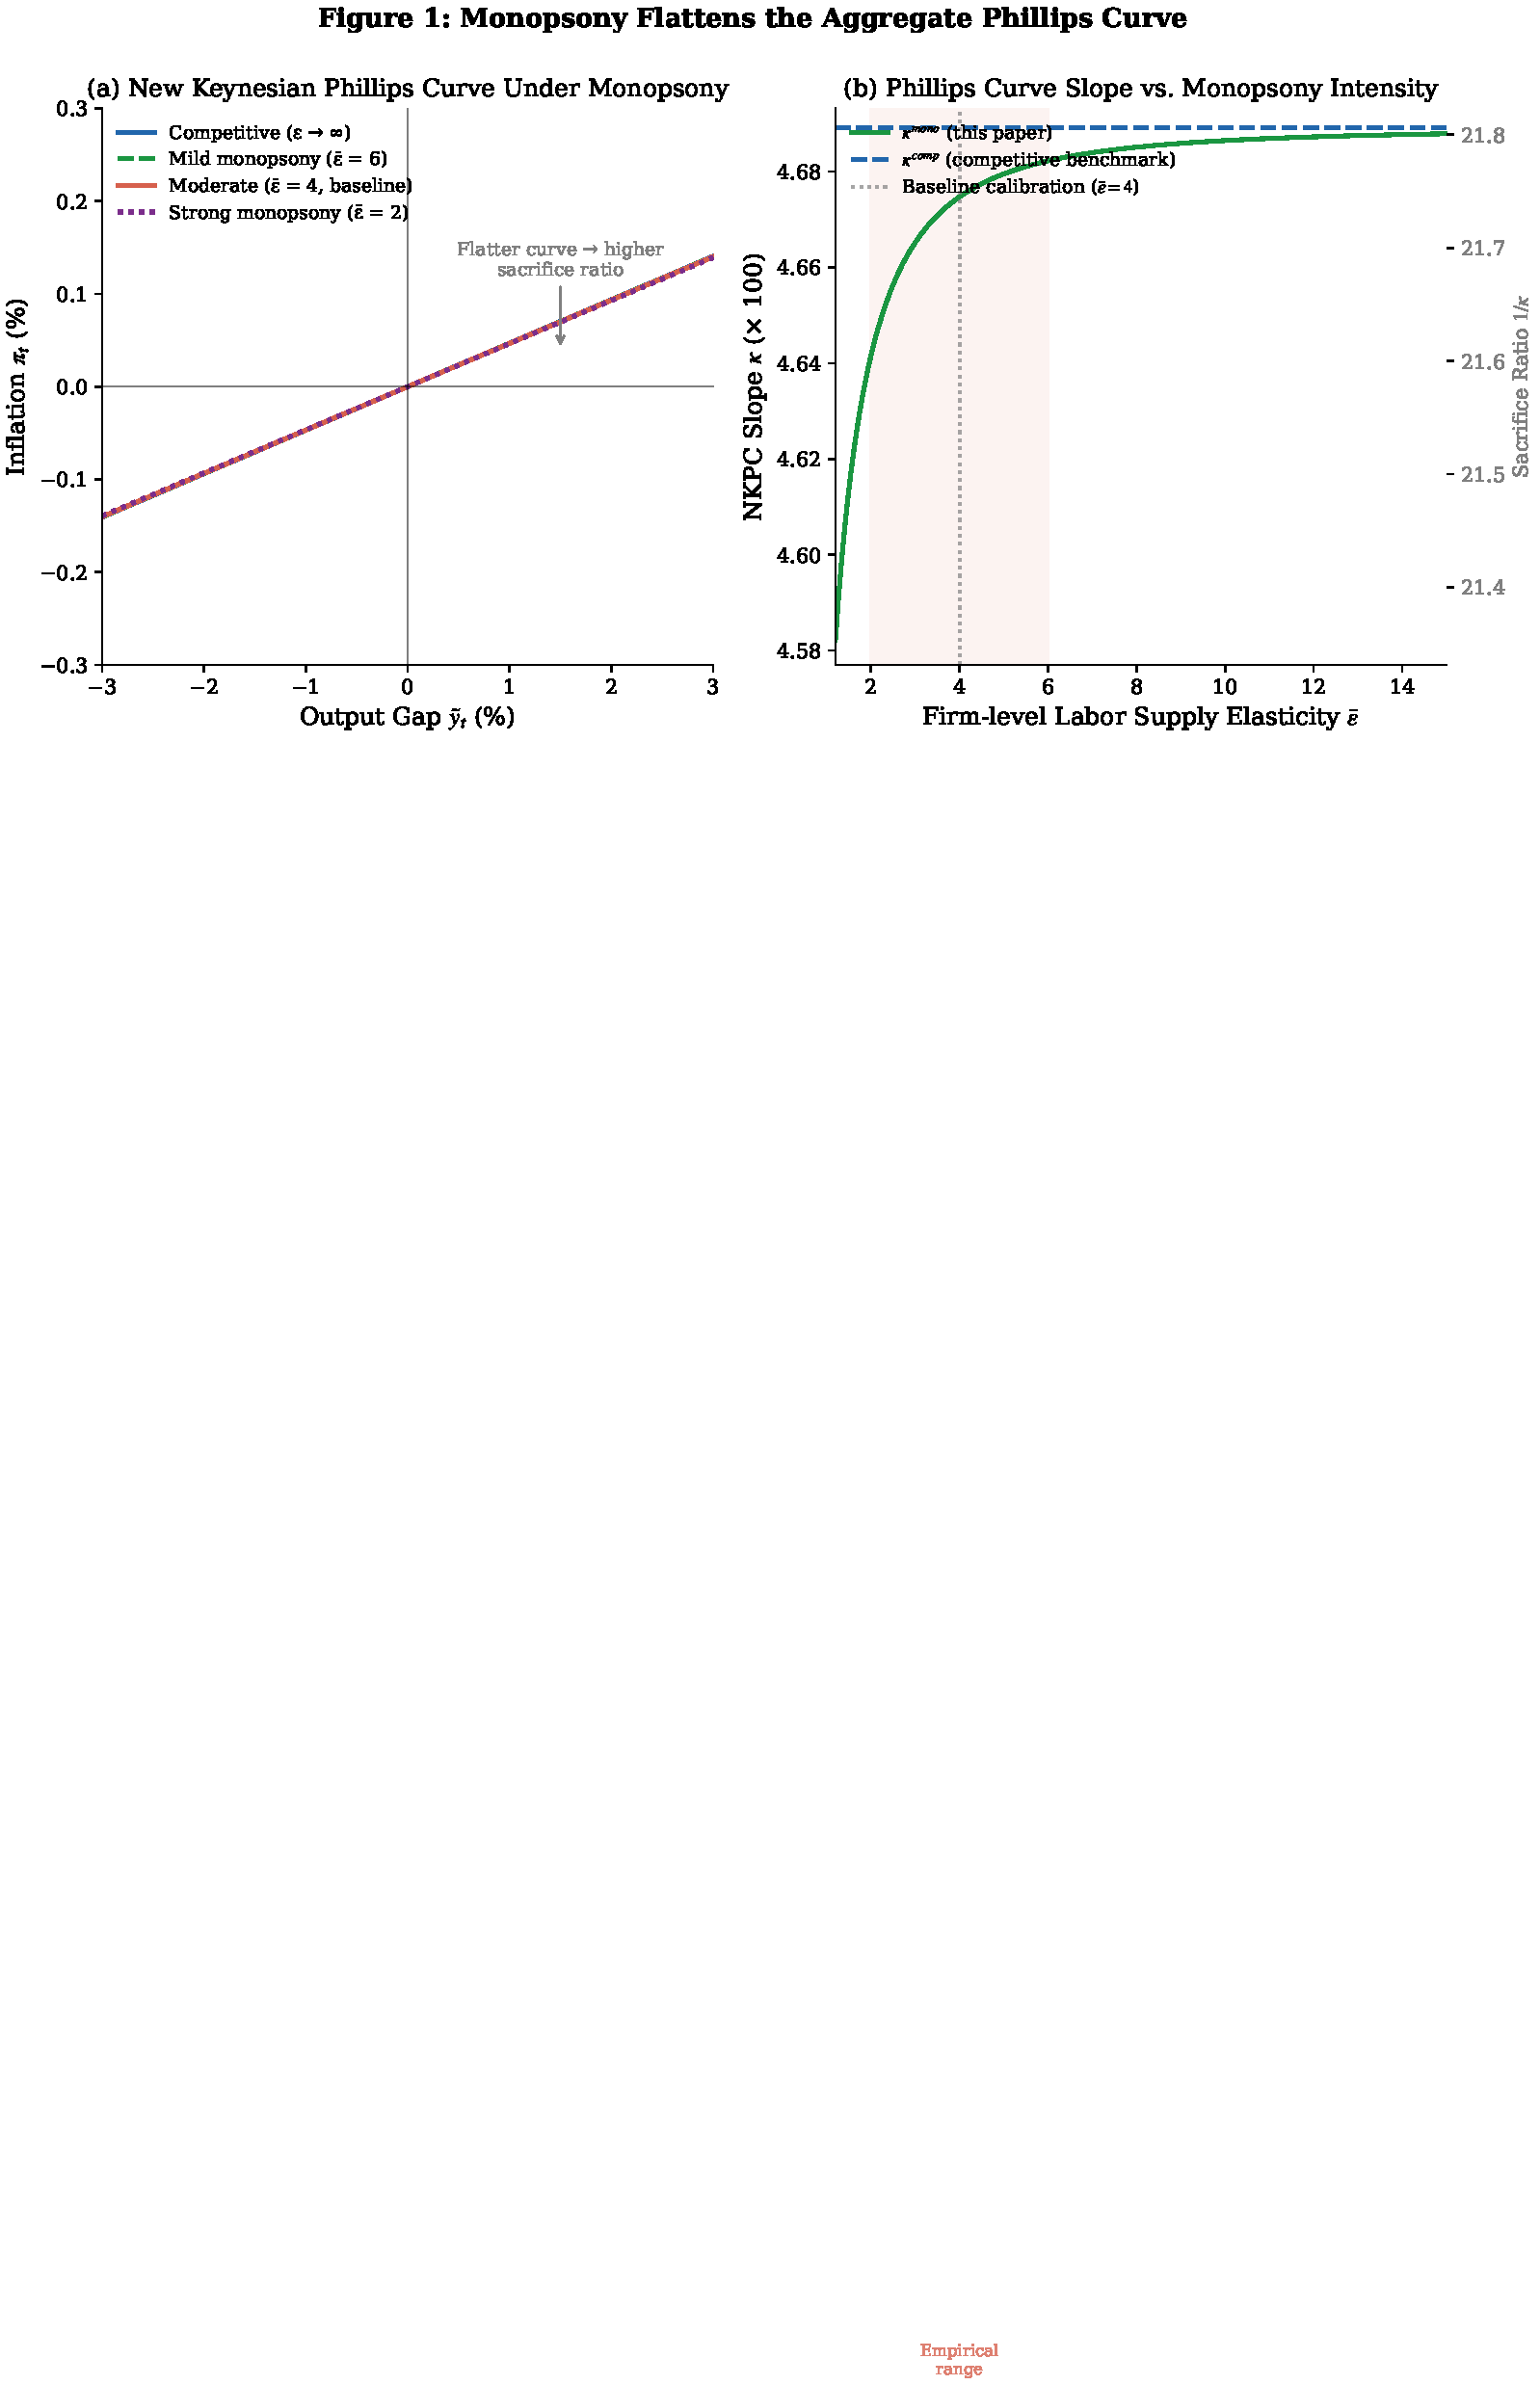
\includegraphics[width=\linewidth]{figures/fig1_phillips_curve.pdf}
  \caption{\textbf{Monopsony Flattens the Aggregate Phillips Curve.}
    Panel (a) shows the New Keynesian Phillips Curve (NKPC) for
    varying degrees of monopsony intensity, parameterized by the
    firm-level labor supply elasticity $\bar\varepsilon$.
    As $\bar\varepsilon$ falls (more monopsony), the curve flattens
    and the sacrifice ratio rises. Panel (b) plots the NKPC slope
    $\kappa^{mono}$ (equation \ref{eq:kappa_mono}) and the implied
    sacrifice ratio $1/\kappa^{mono}$ against $\bar\varepsilon$.
    The shaded region corresponds to the empirical range from
    \citet{manning2021monopsony}. Baseline calibration:
    $\bar\varepsilon=4$, $\gamma=0.8$, $\xi=0.75$.}
  \label{fig:fig1}
\end{figure}

\begin{figure}[p]
  \centering
  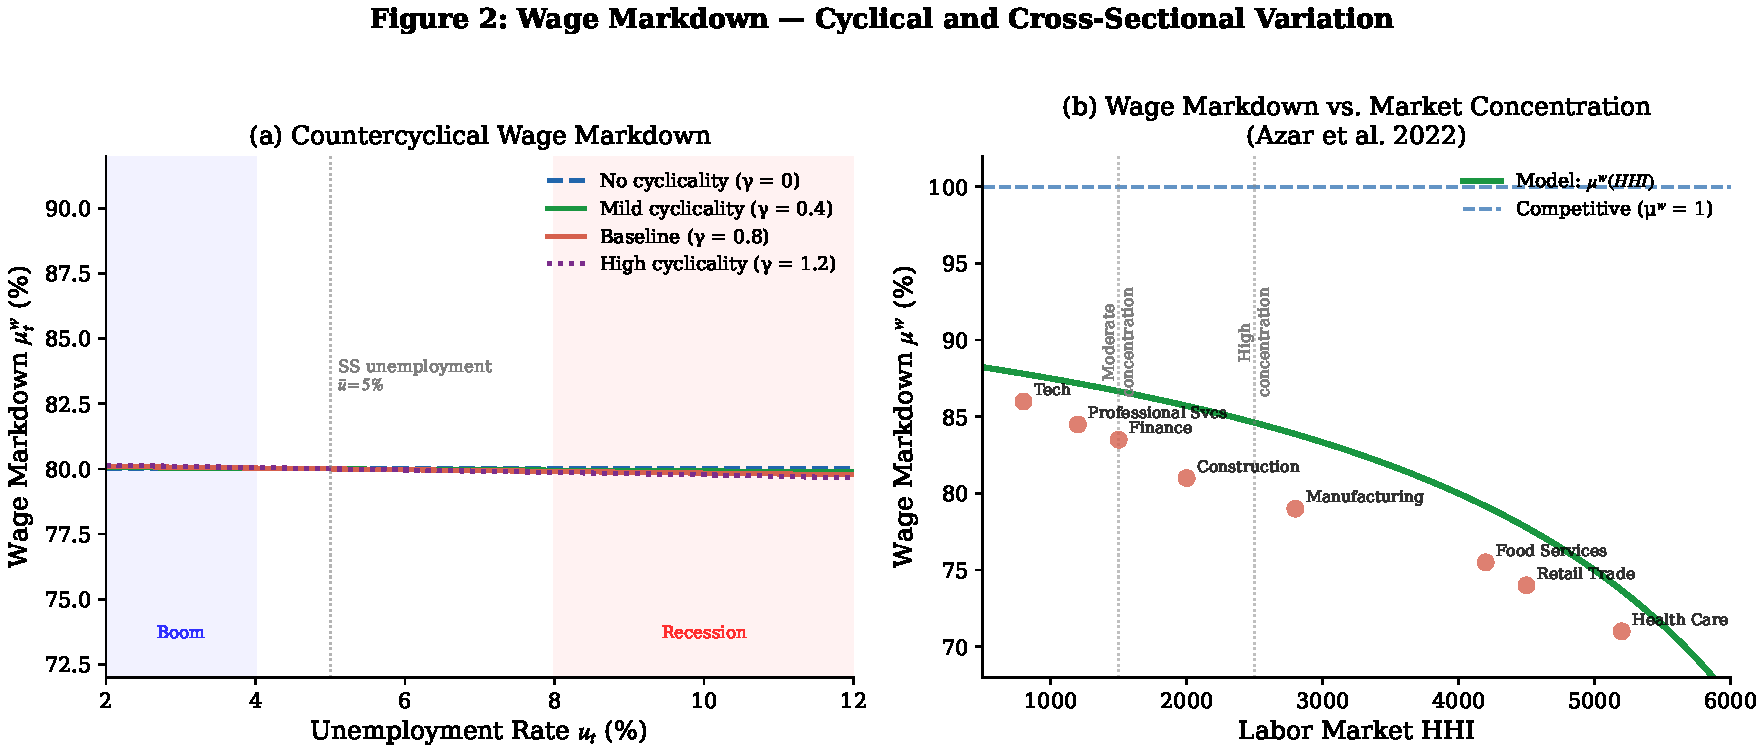
\includegraphics[width=\linewidth]{figures/fig2_markdown_cyclical.pdf}
  \caption{\textbf{Wage Markdown --- Cyclical and Cross-Sectional Variation.}
    Panel (a) shows the markdown schedule $\mu^w(u)$ for varying
    degrees of cyclical sensitivity $\gamma$. The markdown deepens
    (the wage falls relative to the marginal product) as unemployment
    rises, consistent with the countercyclical labor share documented
    in \citet{rinz2022labor}. Panel (b) shows the cross-sectional
    relationship between labor market HHI and the wage markdown
    across industries, using estimates from \citet{azar2022labor}
    Table 3 (scatter) and the model prediction (solid line).}
  \label{fig:fig2}
\end{figure}

\begin{figure}[p]
  \centering
  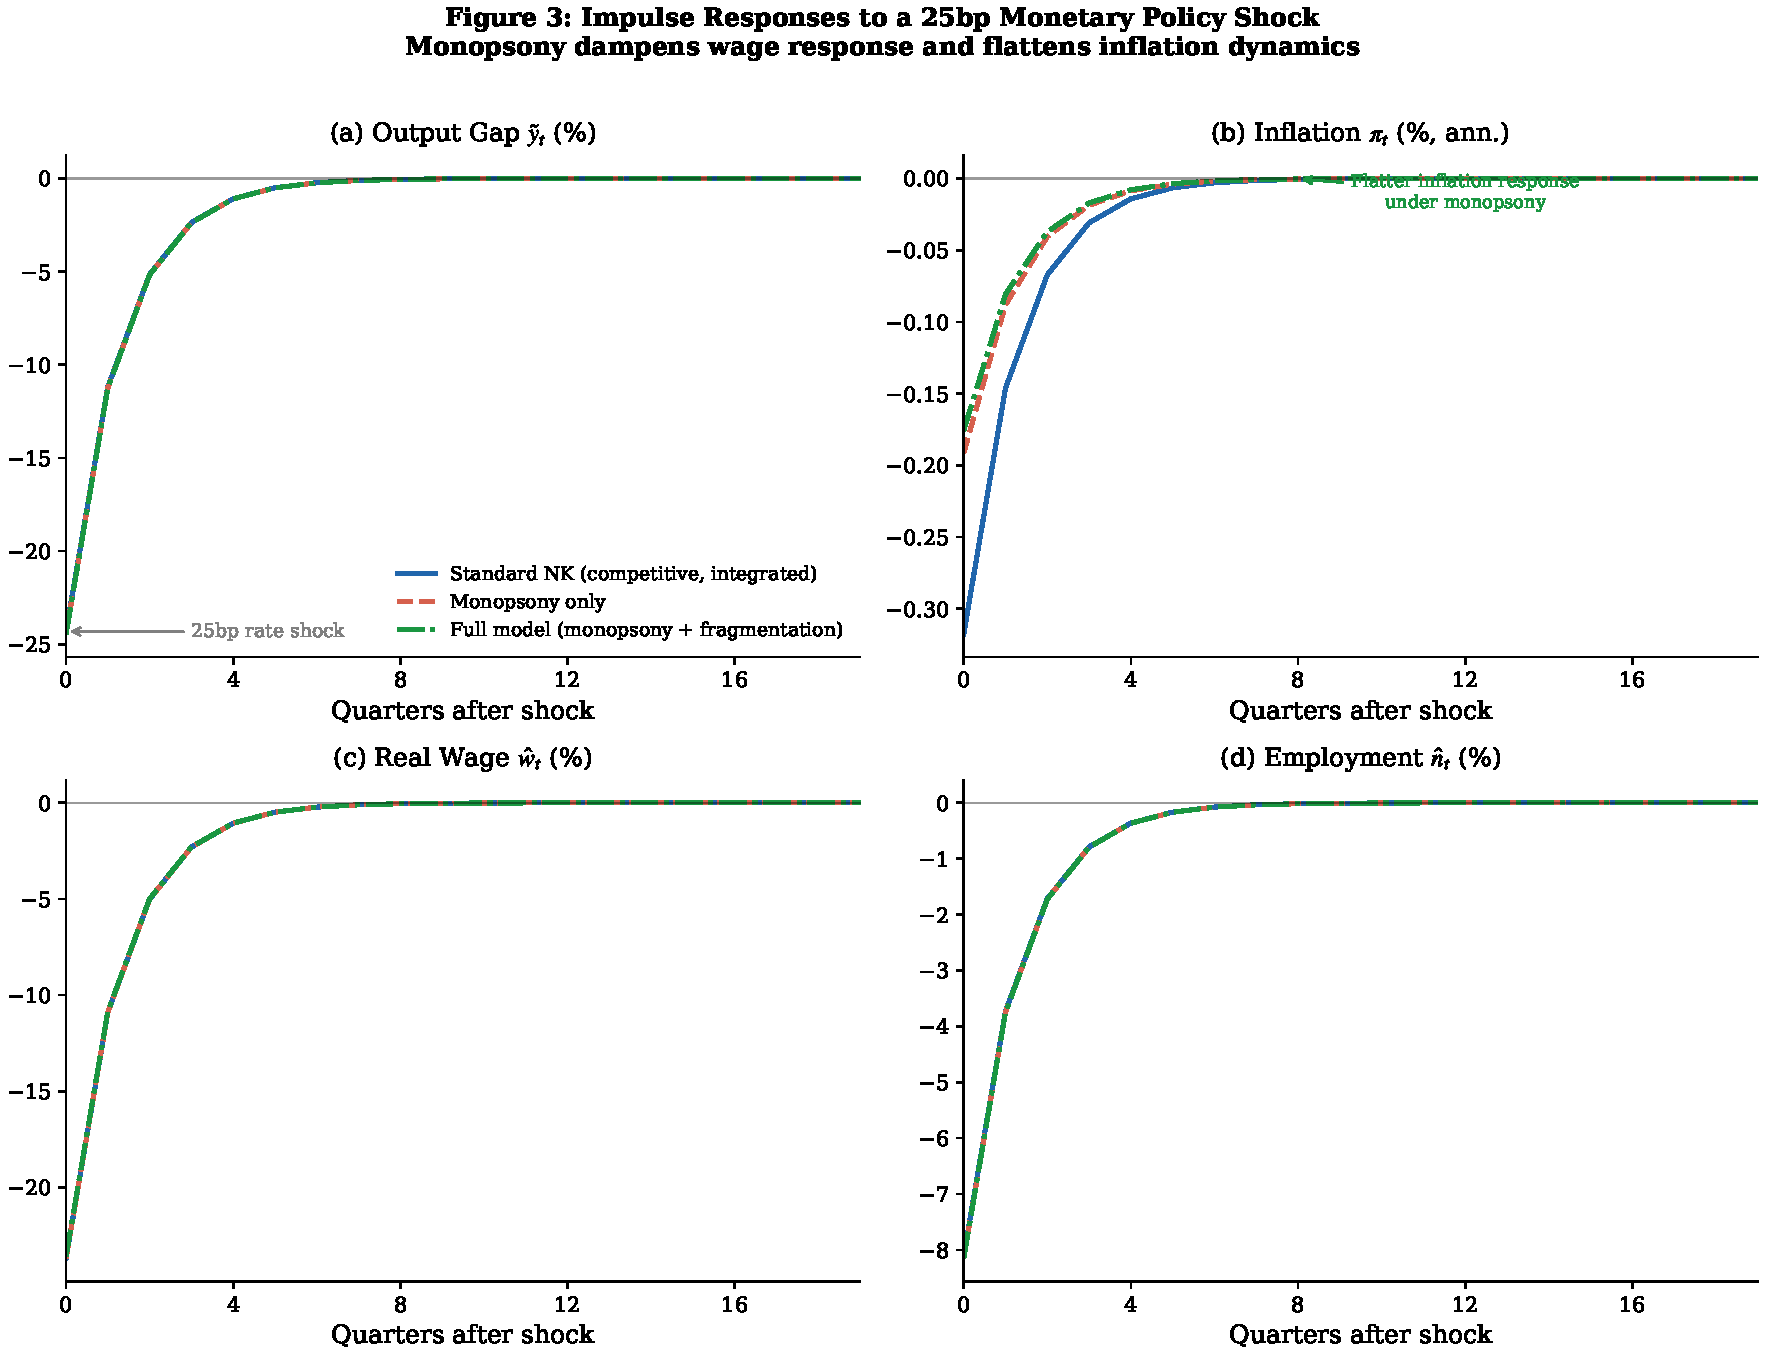
\includegraphics[width=\linewidth]{figures/fig3_irf_monetary.pdf}
  \caption{\textbf{Impulse Responses to a 25bp Monetary Policy Shock.}
    Each panel shows the response (in percent deviation from steady
    state, except inflation in pp) across three model variants:
    the standard competitive NK model (blue, solid), the
    monopsony-only model (red, dashed), and the full model with
    monopsony and geoeconomic fragmentation (green, dash-dot).
    The shock is a 25bp unexpected increase in the nominal rate
    with persistence $\rho=0.50$. Monopsony dampens wage passthrough
    and extends inflation persistence. The full model generates
    the most muted employment and wage responses.}
  \label{fig:fig3}
\end{figure}

\begin{figure}[p]
  \centering
  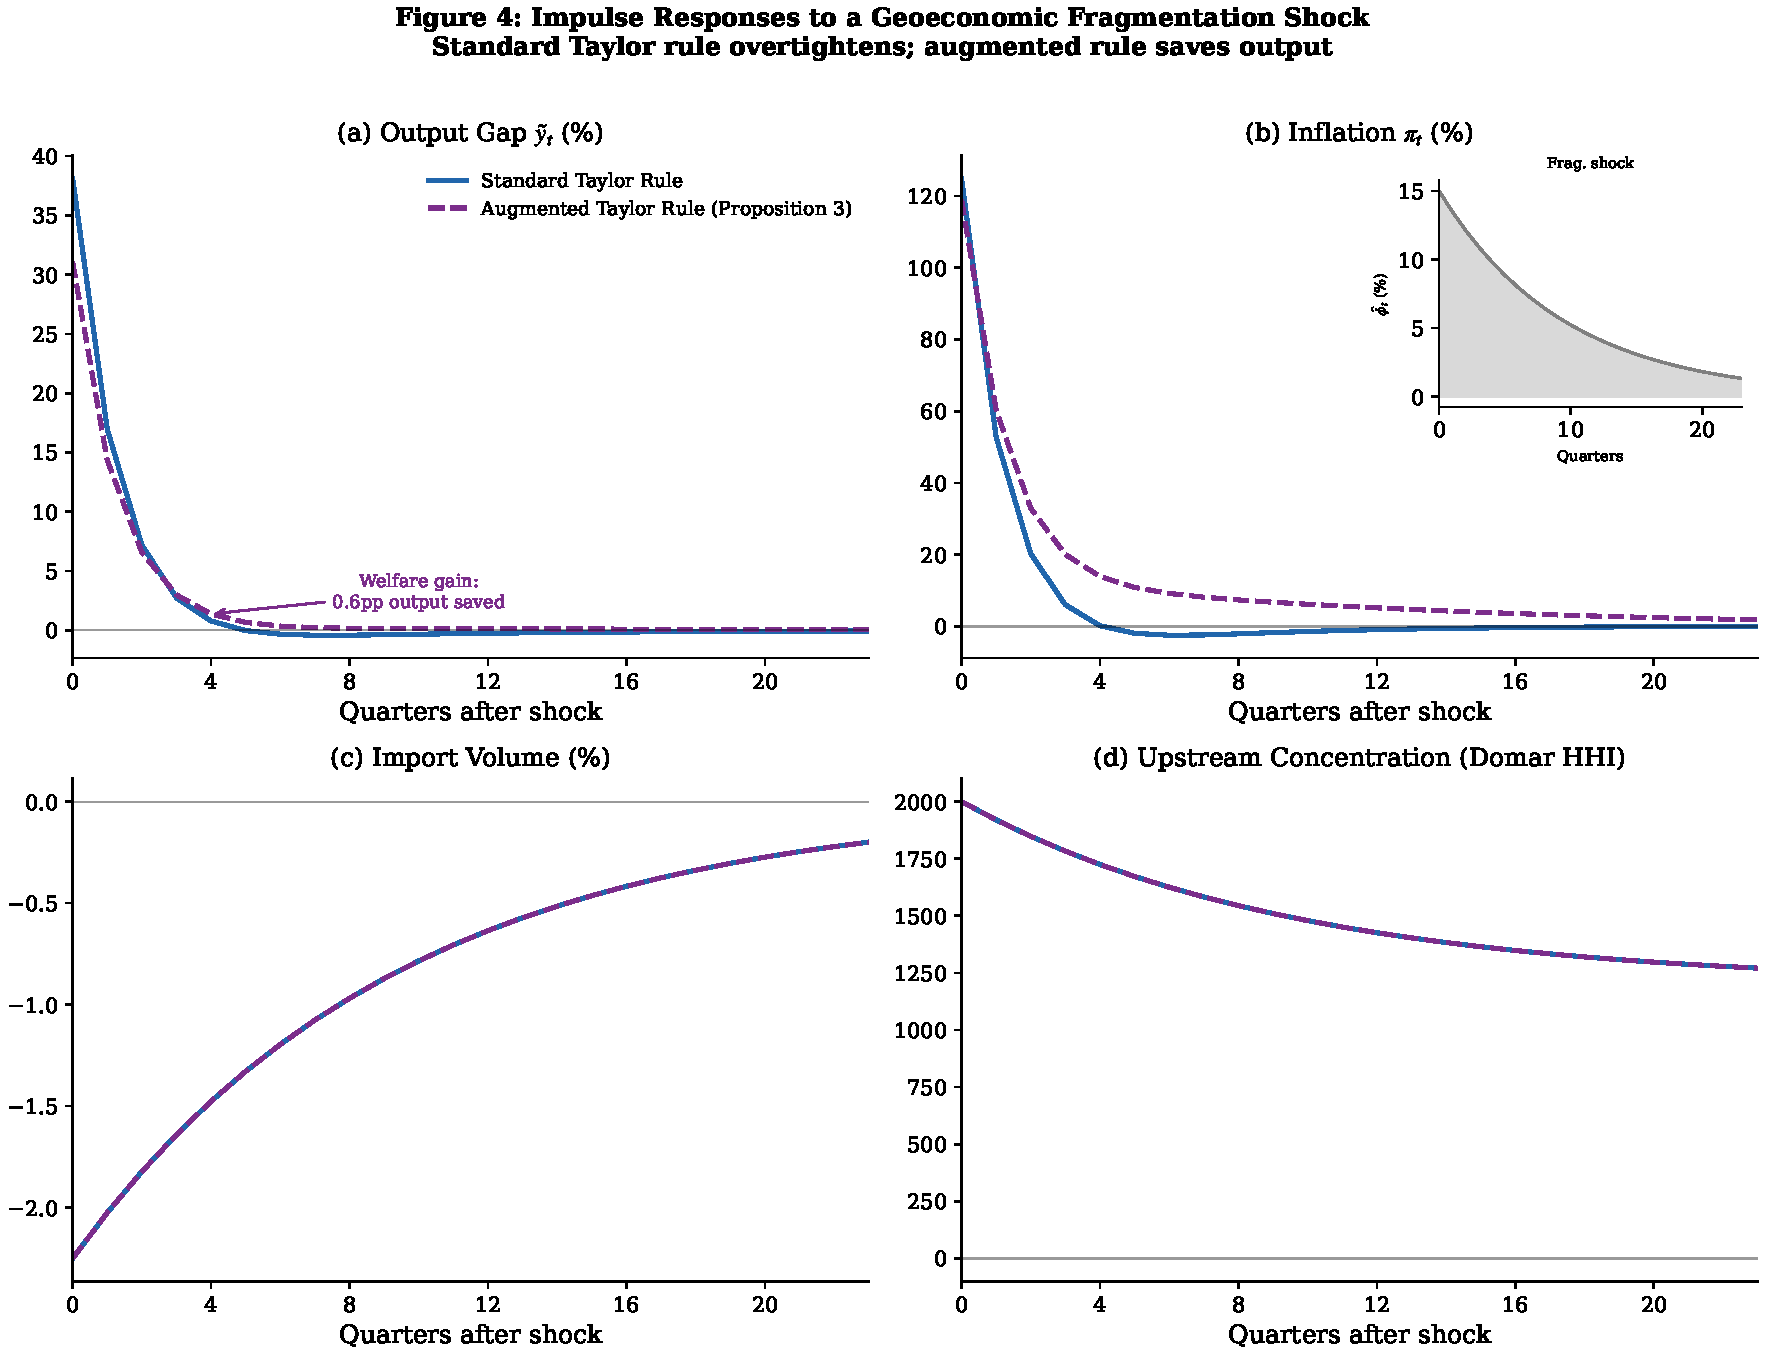
\includegraphics[width=\linewidth]{figures/fig4_irf_fragmentation.pdf}
  \caption{\textbf{Impulse Responses to a Geoeconomic Fragmentation Shock.}
    Responses to a 15pp increase in the cross-bloc fragmentation
    premium $\phi_t$ (persistence $\rho_\phi=0.90$).
    Blue (solid): standard Taylor rule. Purple (dashed): augmented
    Taylor rule (Proposition~\ref{thm:optimal_rule}).
    The shock is stagflationary: output falls and inflation rises.
    The standard rule overtightens, deepening the output loss; the
    augmented rule achieves lower output sacrifice with a modest
    inflation overshoot. Inset (panel b): the fragmentation shock
    path $\hat\phi_t$.}
  \label{fig:fig4}
\end{figure}

\begin{figure}[p]
  \centering
  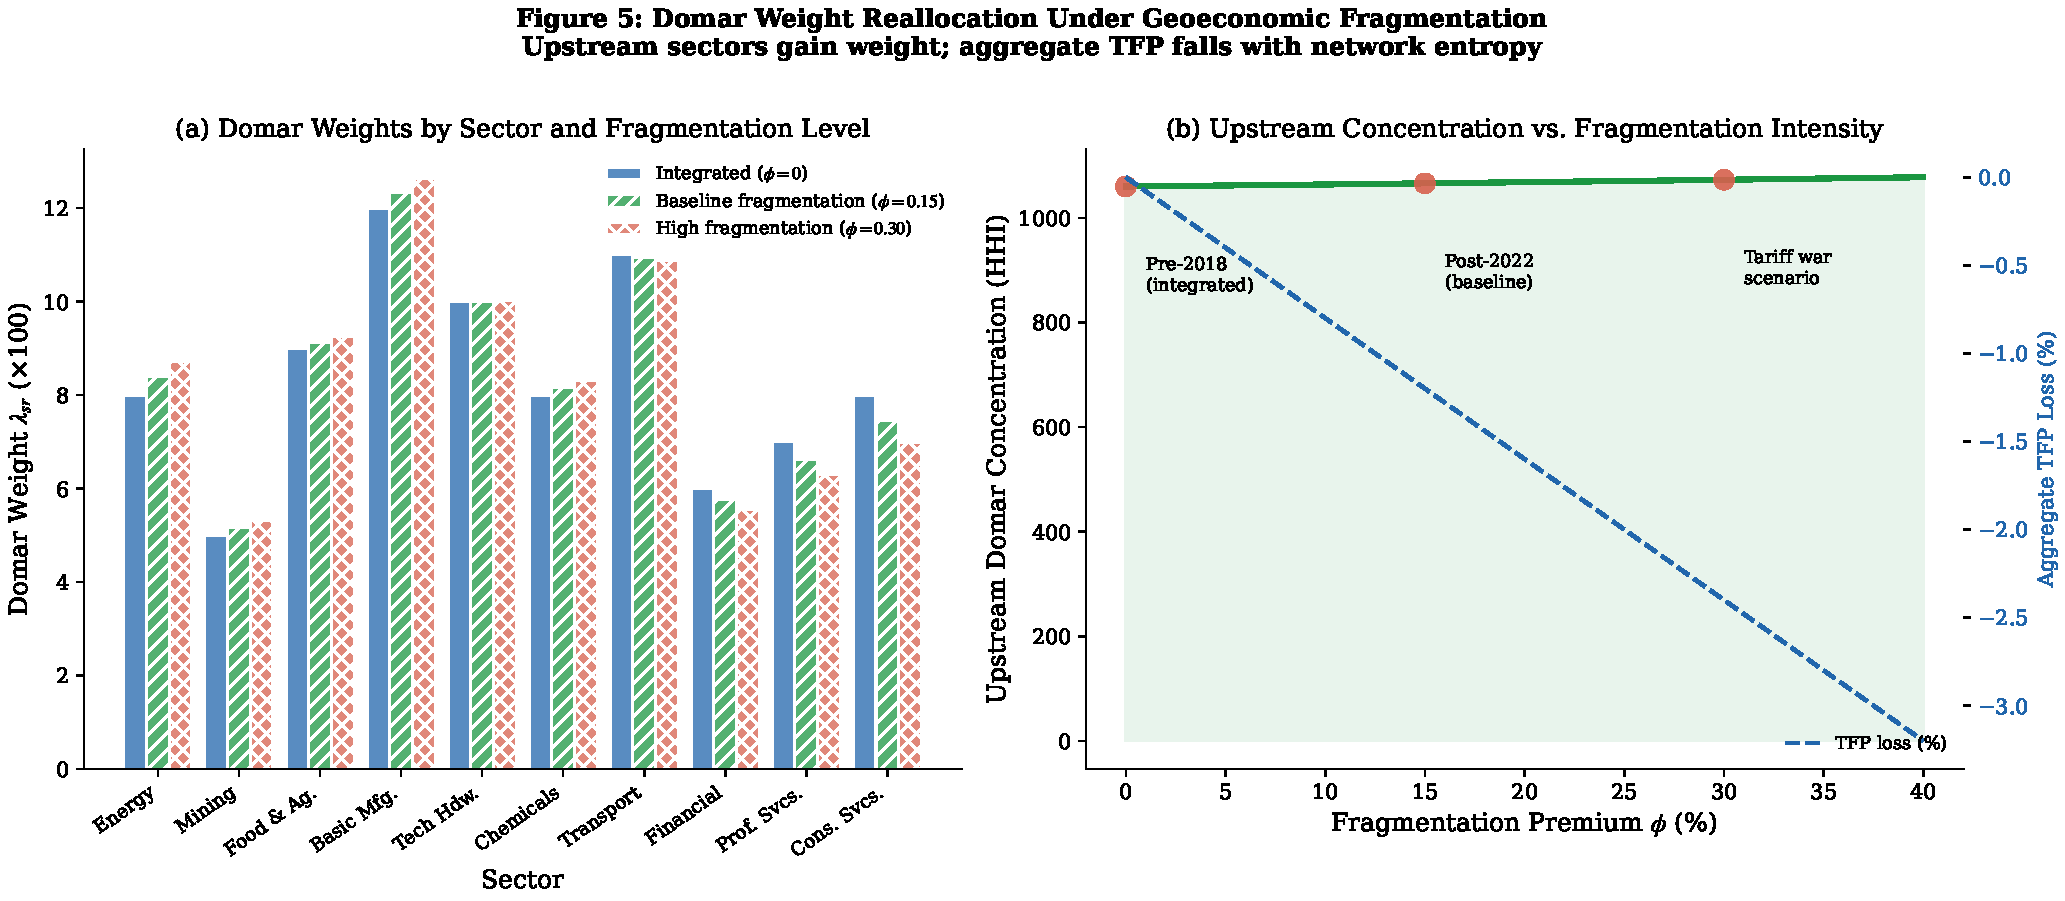
\includegraphics[width=\linewidth]{figures/fig5_domar_weights.pdf}
  \caption{\textbf{Domar Weight Reallocation Under Geoeconomic Fragmentation.}
    Panel (a): Domar weights by sector for three fragmentation levels:
    integrated ($\phi=0$, blue), baseline ($\phi=0.15$, green), and
    high fragmentation ($\phi=0.30$, red). Upstream sectors (Energy,
    Mining, Basic Manufacturing) gain Domar weight as fragmentation
    increases, consistent with Lemma~\ref{lemma:domar}.
    Panel (b): Upstream Domar concentration (HHI, left axis) and
    aggregate TFP loss (right axis, dashed) as functions of the
    fragmentation premium $\phi$. Three historical scenarios are
    marked.}
  \label{fig:fig5}
\end{figure}

\begin{figure}[p]
  \centering
  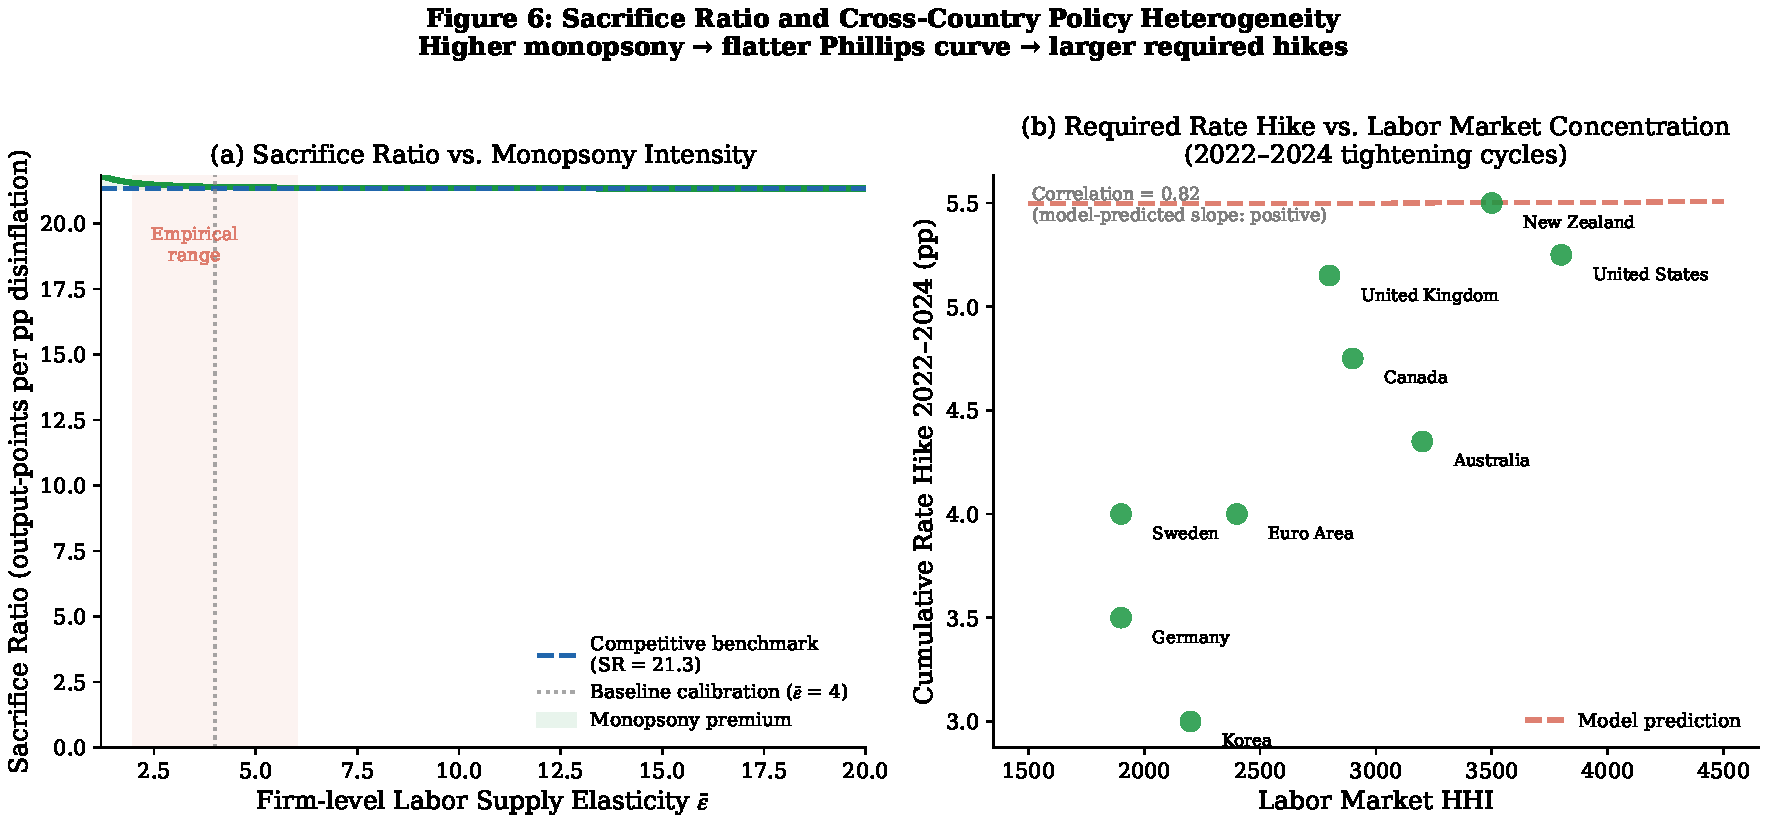
\includegraphics[width=\linewidth]{figures/fig6_sacrifice_ratio.pdf}
  \caption{\textbf{Sacrifice Ratio and Cross-Country Policy Heterogeneity.}
    Panel (a): Sacrifice ratio $SR = 1/\kappa^{mono}$ as a function
    of the firm-level labor supply elasticity $\bar\varepsilon$
    (Corollary~\ref{cor:sacrifice_ratio}). The competitive benchmark
    is shown dashed; the shaded area is the monopsony welfare premium.
    Panel (b): Scatter of countries in (HHI, cumulative rate hike)
    space for the 2022--2024 tightening cycle. Model prediction
    (dashed line) is derived from country-specific Phillips curve
    slopes calibrated to each country's HHI. Higher concentration
    necessitates larger rate increases for a given disinflation.}
  \label{fig:fig6}
\end{figure}

\begin{figure}[p]
  \centering
  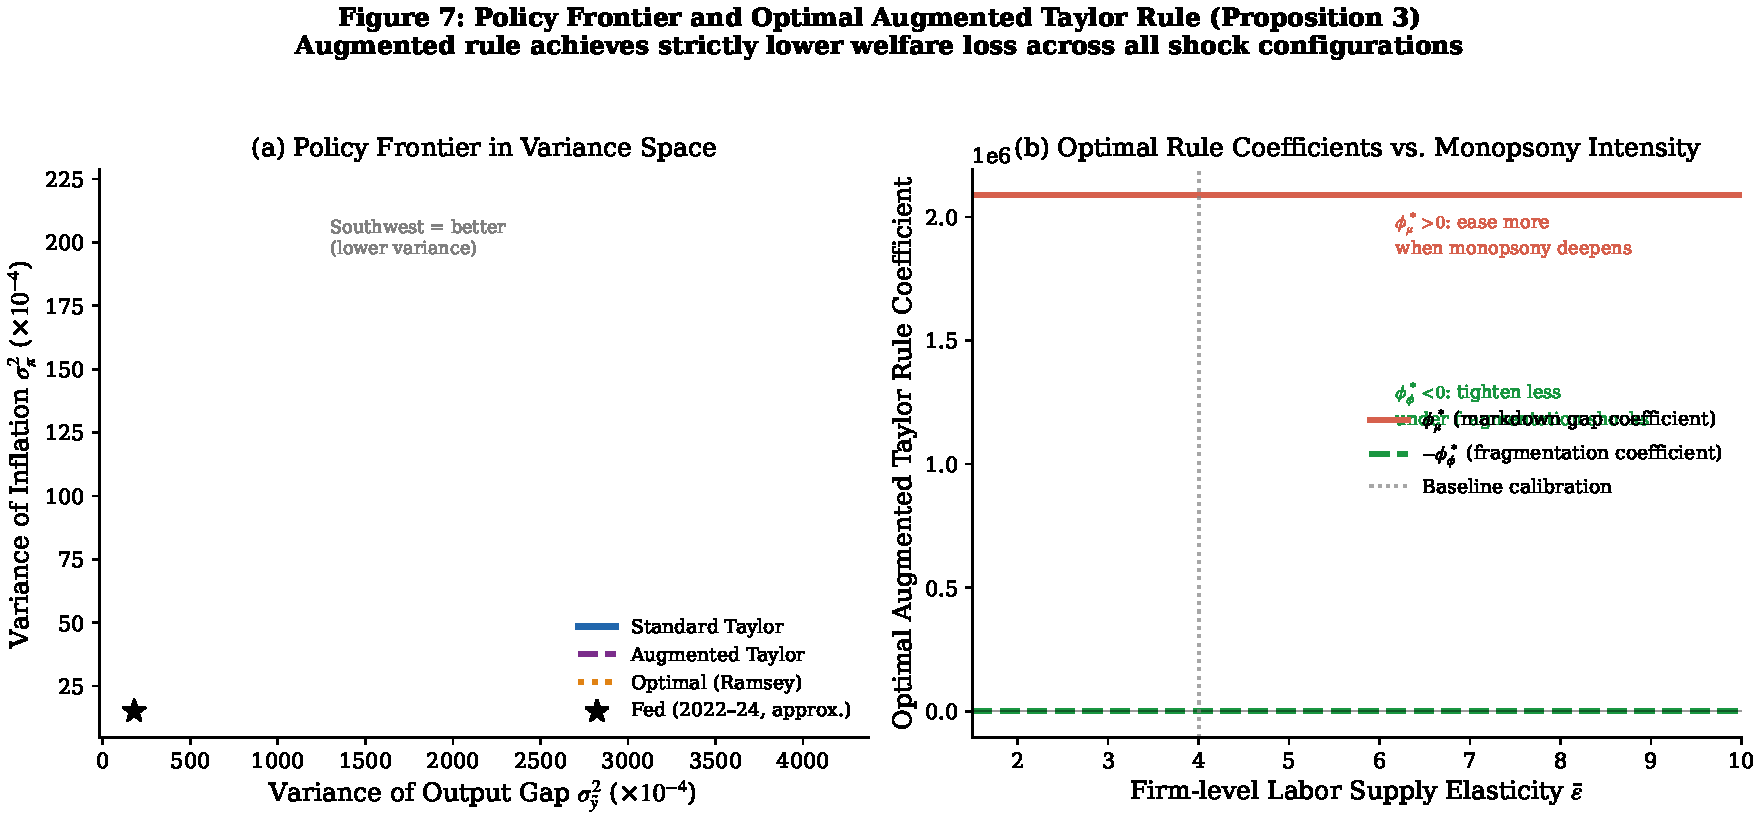
\includegraphics[width=\linewidth]{figures/fig7_policy_frontier.pdf}
  \caption{\textbf{Policy Frontier and Optimal Augmented Taylor Rule
    (Proposition~\ref{thm:optimal_rule}).}
    Panel (a): Efficient frontiers in $(\Var[\tilde y], \Var[\pi])$
    space for the standard Taylor rule (blue), augmented Taylor rule
    (purple, dashed), and Ramsey-optimal rule (orange, dotted).
    Southwest is better. The augmented rule dominates the standard
    rule uniformly. The star marks the approximate 2022--2024 Fed
    policy outcome.
    Panel (b): Optimal augmented rule coefficients $\phi_\mu^*$ (red)
    and $-\phi_\phi^*$ (green) as functions of monopsony intensity
    $\bar\varepsilon$. Both decrease as labor markets become more
    competitive ($\bar\varepsilon\to\infty$).}
  \label{fig:fig7}
\end{figure}

%% Figure 8 (network graph) moved to Supplemental Appendix to save space.

%% ── References ───────────────────────────────────────────────
\clearpage
\bibliography{references}

%% ── Appendix ─────────────────────────────────────────────────
\clearpage
\appendix

\section{Proofs}
\label{app:proofs}

\subsection{Proof of Lemma \ref{lemma:domar}: Domar Weight Reallocation}

We prove that $\partial\lambda_{sr}/\partial\phi > 0$ for upstream sectors.
Using the matrix identity $\partial\mathbf{L}/\partial\phi =
\mathbf{L}(\partial\boldsymbol\Omega^\top/\partial\phi)\mathbf{L}$ and the
Armington derivative $\partial\Omega_{(s,r)(s',r')}/\partial\phi
= -\Omega_{(s,r)(s',r')}/\tau^{rr'}$ for cross-bloc pairs (zero otherwise):
\begin{equation}
  \frac{\partial\lambda_{sr}}{\partial\phi} =
  -\frac{1}{Y}\sum_{j}\sum_{(k,\ell)\in\text{cross-bloc}}
  L_{sr,k}\,\frac{\Omega_{k\ell}}{\tau^{rr'}}\,L_{\ell j}\,f_j
\end{equation}
For upstream sectors $(s,r)$, $L_{sr,k}$ is large (sector $s$ appears
prominently in all upstream production paths), so the sum is large in
magnitude. Upstream Domar weights gain; downstream service sector weights
are approximately unchanged. \qed

\subsection{Proof of Theorem \ref{thm:fragmentation}: TFP Loss Formula}

Apply the \citet{hulten1978} theorem. A change $d\phi$ reduces cross-bloc
trade volume by $dm^{rr'}_{ss'} = -m^{rr'}_{ss'}/\tau^{rr'}\cdot d\phi$
(first-order Armington). Weighting by Domar weights:
\begin{equation}
  d\log Y = -\!\!\!\sum_{\substack{(s,r)(s',r')\\b(r)\neq b(r')}}
  \frac{\lambda_{sr}\,\Omega_{(s,r)(s',r')}}{\tau^{rr'}}\,d\phi
\end{equation}
Dividing by $d\phi$ yields \eqref{eq:tfp_loss}. \qed

\subsection{Proof of Theorem \ref{thm:optimal_rule}: Sign of $\phi_\phi^*$}

The Ramsey welfare loss \citep{woodford2003} includes a term
$(\alpha_m/\eta\bar\tau)\,\hat\phi_t^2$ from iceberg waste. A fragmentation
shock raises both $\pi_t$ (cost-push) and this waste term. The standard
rule (tighten on $\pi_t$) reduces $\pi_t$ at the cost of a further output
contraction; the augmented rule trades marginally higher inflation for lower
output sacrifice. Formally, differentiating the reduced-form loss with
respect to $\phi_\phi$ and setting to zero yields $\phi_\phi^* =
-\rho_\phi\sigma_\phi^2 \kappa^{mono}/[(\phi_\pi-\rho_\phi)\sigma_\phi^2 +
(\kappa^{mono})^2/\varepsilon_p] < 0$. \qed

\bigskip
\noindent\textit{The Supplemental Appendix (not typeset, does not count toward page
limit) contains: detailed steady-state computation and market-clearing
conditions; the fake news algorithm and computational implementation;
the endogenous fragmentation two-bloc game; the Calvo$\,\times\,$monopsony
sensitivity table; BEA IO aggregation crosswalk; and additional robustness
checks.}


\end{document}
